\documentclass[11pt]{article}

% ------------------------------------------------
% PACKAGES
% ------------------------------------------------
\usepackage{amsmath, amssymb, amsthm}
\usepackage{geometry}
\usepackage{hyperref}
\usepackage{bm}
\usepackage{mathrsfs}
\usepackage{setspace}
\usepackage{lipsum}
\pdfoutput=1
%\usepackage{geometry}
\geometry{margin=1in}
\usepackage{times}
\usepackage{microtype}
%\usepackage{hyperref}
\geometry{a4paper, margin=1in}
\onehalfspacing
% ---------- Encoding & language ----------
\usepackage[T1]{fontenc}
\usepackage[utf8]{inputenc}
\usepackage[english]{babel}

% ---------- Fonts & math ----------
\usepackage{lmodern}
\usepackage{amsmath,amssymb,amsfonts}
\usepackage{siunitx}

% ---------- Page layout ----------
\usepackage{geometry}
\geometry{margin=1in}

% ---------- Tables, captions ----------
\usepackage{booktabs}
\usepackage{caption}
\usepackage{seqsplit}


% ---------- Links ----------
\usepackage{hyperref}
\hypersetup{
	colorlinks=true,
	linkcolor=blue,
	citecolor=blue,
	urlcolor=blue
}

\usepackage{amsmath, amsthm, amssymb}
\usepackage{tikz}
\usetikzlibrary{arrows.meta,calc,decorations.markings,patterns}
\theoremstyle{definition}
\newtheorem{definition}{Definition}[section]
\theoremstyle{plain}
\newtheorem{theorem}{Theorem}[section]
\newtheorem{lemma}{Lemma}[section]
\theoremstyle{remark}
\newtheorem*{remark}{Remark}
\newtheorem{corollary}[theorem]{Corollary}
\newtheorem{proposition}{Proposition}[section]

\usepackage{tikz}
\usepackage{pgfplots}
\pgfplotsset{compat=1.18}

\usetikzlibrary{
	calc,
	decorations.pathmorphing,
	decorations.markings,
	shapes,
	arrows.meta,
	angles,
	quotes,
	patterns,
	intersections,
	math
}
\usepackage{tikz}
\usetikzlibrary{calc,arrows.meta,decorations.markings}

\tikzset{
	>=latex,                  % lijepi strelice
	spiral/.style={blue, thick},
	curve/.style={smooth, thick}
}

\setcounter{tocdepth}{2}


% ---------- Simple macros ----------
\newcommand{\PhiConst}{\varphi}
\newcommand{\deltam}{\Delta m}
\newcommand{\QCOtwo}{Q_{\mathrm{CO_2}}}
\newcommand{\QHtwoO}{Q_{\mathrm{H_2O}}}

\newcommand{\KGB}{Kolarec--Gauss--Bonnet }
\newcommand{\KEGB}{Kolarec--Einstein--Gauss--Bonnet }
\newcommand{\PG}{\Phi\text{--Gauss--Bonnet}}
\newcommand{\PE}{\Phi\text{–Einstein}}


\usepackage{microtype} % perfect kerning and spacing
\usepackage{times}     % more compact, professional font
\usepackage{titlesec}  % fine-tuned section headers
\titleformat{\section}{\bfseries\large}{\thesection}{1em}{}
\usepackage{csquotes}
\usepackage{enumerate}







% ------------------------------------------------
% TITLE PAGE
% ------------------------------------------------
	\title{\textbf{Kolarec--Gauss--Bonnet and Kolarec--Einstein--Gauss--Bonnet Geometry:\\
		A Unified $\Phi$--Resonant Curvature Framework}}

\author{Robert Kolarec\\
	Independent Researcher, Zagreb, Croatia, EU\\[0.2cm]
	\small Email: {robert.kolarec@gmail.com}\\
	\texttt{DOI: 10.5281/zenodo.17636104 }}
	
\date{17 November 2025}

\begin{document}
	\maketitle
	\tableofcontents
	\bigskip
	

	% ------------------------------------------------
	% ABSTRACT
	% ------------------------------------------------
	\section{abstract}
	
	\begin{abstract}
		I introduce a $\Phi$–spiral geometric deformation that produces a nontrivial 
		Gauss--Bonnet contribution in four dimensions without dimensional continuation. 
		The resulting Kolarec--Einstein--Gauss--Bonnet equation suggests a unified 
		differential--geometric structure with potential implications across physical 
		scales, from subatomic to cosmological regimes. The construction is 
		mathematically explicit, uses no regularization procedure, and yields a finite 
		boundary term responsible for dynamical corrections to Einstein gravity in 4D. 
		I also outline possible geometric parallels with resonant molecular helices, 
		leaving quantitative biological analysis for future work.
	\end{abstract}
	
	\noindent\textbf{Keywords:} Gauss--Bonnet geometry, Einstein--Gauss--Bonnet gravity, golden ratio, 
	logarithmic spiral, Kolarec--Planck operator, $\Phi$--Hilbert space, resonant curvature.
	
	\newpage
	
	% ------------------------------------------------
	% SECTION 1 — INTRODUCTION
	% ------------------------------------------------
	
	\section{Introduction}
	
	The purpose of this work is to unify several independent mathematical and physical structures 
	I have previously introduced---including the $\Phi$--Fourier transform, the Kolarec--Planck operator, 
	the $\Phi$--Hilbert space, and the exponential kernel of the golden ratio spiral---within a single 
	curvature framework built upon a 4D generalization of Gauss--Bonnet geometry.
	
	Classically, the Gauss--Bonnet functional in four dimensions is topological and therefore dynamically 
	trivial; it does not contribute to the Einstein field equations. 
	Yet this same functional naturally encodes global geometric information about a manifold. 
	What I show in this work is that, once the geometry is expressed in terms of a logarithmic spiral, 
	with exponential growth rate 
	$\alpha_\Phi = \frac{\ln\Phi}{2\pi}$ 
	and spiral Jacobian 
	$J_\Phi = 1 + \alpha_\Phi^2$, 
	the Gauss--Bonnet functional becomes fully dynamical even in 4D.
	
	This is the key step that allows me to construct the Kolarec--Gauss--Bonnet and 
	Kolarec--Einstein--Gauss--Bonnet frameworks. 
	These new structures suggest a common geometric mechanism underlying multiple 
	resonant, geometric, thermodynamic, and quantum phenomena through 
	the single damping factor:
	\[
	e^{-2\pi\alpha_\Phi} = \frac{1}{\Phi}.
	\]
	
	I show that this factor appears universally, not only in curvature, but also in:
	\begin{itemize}
		\item the $\Phi$--Fourier transform,
		\item the Kolarec--Planck exponential operator,
		\item the $\Phi$--Maxwell--Boltzmann distribution,
		\item the Euler kernel of the golden ratio spiral,
		\item the $\Phi$--Hilbert inner product,
		\item the quantized glueball spectrum,
		\item orbital resonance structures,
		\item and the DNA/RNA resonant model.
	\end{itemize}
	
	This universality suggests the existence of a deeper geometric principle, which I formalize in this work.
	This construction appears to provide the first explicit 4D formulation in which 4D Gauss–Bonnet geometry becomes dynamically relevant without dimensional continuation, auxiliary fields, or regularization procedures.
	
	\section{Notation}
	\addcontentsline{toc}{section}{Notation}
	
	Throughout this work $g_{\mu\nu}$ denotes the original metric, 
	$g^{(\Phi)}_{\mu\nu}$ its $\Phi$–deformation, 
	$G$ the normalized Gauss--Bonnet scalar, 
	$G_{\Phi}$ its $\Phi$--scaled version, 
	$\alpha_{\Phi}$ the spiral damping constant, 
	$\widetilde{G}$ the conventional unnormalized Gauss--Bonnet density, 
	and $\chi(M)$ the Euler characteristic of a closed manifold $M$.
	
	
	
	% ------------------------------------------------
	% SECTION 2 — BACKGROUND
	% ------------------------------------------------
	
	\section{Background and Motivation}

	The logarithmic spiral
	\[
	r(\theta)=r_0\, e^{\kappa \theta}
	\]
	is the only planar curve whose shape is preserved under radial dilation.  
	The scaling factor associated with a full $2\pi$ rotation satisfies 
	\[
	e^{2\pi\kappa}=\lambda,
	\]
	and the curve is self-similar if and only if $\lambda$ is constant across 
	all scales.  

	Among all $\lambda>1$, the unique choice that minimizes curvature distortion, 
	maximizes geometric self-similarity, and produces a scale-invariant spiral is 
	the golden ratio:
	\[
	\lambda=\Phi=\frac{1+\sqrt{5}}{2}.
	\]
	This singles out the constant
	\[
	\kappa = \frac{\ln\Phi}{2\pi}=\alpha_\Phi,
	\]
	which plays the role of a universal geometric damping rate.  
	The identity
	\[
	e^{2\pi\alpha_\Phi}=\Phi
	\]
	is therefore not arbitrary: it expresses the only dilation factor for which a 
	logarithmic spiral reproduces itself exactly after each full rotation.

	\begin{remark}[Why the Golden Ratio Appears]
	The choice of $\Phi$ is mathematically forced.  
	Among all real scaling constants $\lambda>1$, only the golden ratio 
	simultaneously satisfies:
	\begin{itemize}
		\item scale-invariance of the logarithmic spiral,
		\item exact self-similarity of curvature shells,
		\item the exponential–reciprocal identity 
		$e^{-2\pi\alpha_\Phi} = 1/\Phi$,
		\item minimal distortion of the spiral metric under dilation,
		\item closure of the resonant Gauss--Bonnet identity 
		$\int_M G_\Phi\, dV_\Phi = 2\pi\, \Phi^{\chi(M)}$.
	\end{itemize}
	No other constant preserves geometric, analytic, and topological coherence 
	across these structures.  
	Thus $\Phi$ is not chosen heuristically—it is the unique value for which the 
	entire resonant framework remains internally consistent.
	\end{remark}

	This exponential law reappears throughout all $\Phi$–based operators, damping 
	kernels, and resonant constructions used in this work.  
	The central thesis of this paper is that curvature itself obeys this 
	$\Phi$–spiral scaling law, and that the Gauss--Bonnet functional becomes 
	dynamically nontrivial in four dimensions precisely because of this structure.

	
	\section{Axiom System for the $\Phi$–Spiral Geometry}
	
	\begin{definition}[Spiral Manifold]
		A \emph{$\Phi$–spiral manifold} $(M,g_{\Phi})$ is a smooth 4--manifold $M$ 
		equipped with a metric
		\[
		g_{\Phi} = J_{\Phi}\, g,
		\]
		where $g$ is a classical Lorentzian metric and 
		$J_{\Phi} = 1 + \alpha_{\Phi}^{2}$ is the constant spiral Jacobian induced by the 
		real spiral chart
		\[
		z(T,X) = \exp[(\alpha_{\Phi}+i)T + (-1 + i\alpha_{\Phi})X].
		\]
	\end{definition}
	
	\begin{definition}[$\Phi$–Damping]
		The $\Phi$–damping law is the exponential weight
		\[
		D_{\Phi} = e^{-2\pi\alpha_{\Phi}} = \frac{1}{\Phi},
		\]
		representing one full logarithmic–spiral rotation.
	\end{definition}
	
	\begin{definition}[$\Phi$–Gauss--Bonnet Curvature]
		The $\Phi$–Gauss–Bonnet scalar is defined by
		\[
		G_{\Phi} = 
		\bigl(R^{2} - 4R_{\mu\nu}R^{\mu\nu} + R_{\mu\nu\alpha\beta}R^{\mu\nu\alpha\beta}\bigr)\,
		D_{\Phi}.
		\]
	\end{definition}
	
	\begin{definition}[$\Phi$–Einstein Tensor]
		The $\Phi$–Einstein tensor is
		\[
		G^{(\Phi)}_{\mu\nu} = G_{\mu\nu} + \alpha_{\Phi} H_{\mu\nu},
		\]
		where $H_{\mu\nu}$ is the Gauss–Bonnet tensor.
	\end{definition}
	
	\section*{Notation and Numerical Constants}
	
	For convenience and to ensure numerical consistency across all calculations, 
	we collect here the fundamental constants used throughout the 
	Kolarec–Gauss–Bonnet and Kolarec–Einstein–Gauss–Bonnet framework.
	
	\begin{table}[h!]
		\centering
		\begin{tabular}{ll}
			\toprule
			Quantity & Definition / Numerical Value \\
			\midrule
			Golden ratio 
			& $\displaystyle \Phi = \frac{1+\sqrt{5}}{2} = 1.6180339887\,4989484820\ldots$ \\[4pt]
			
			Inverse golden ratio 
			& $\displaystyle \Phi^{-1} = 0.6180339887\,4989484820\ldots$ \\[4pt]
			
			Spiral exponent 
			& $\displaystyle \alpha_\Phi = \frac{\ln \Phi}{2\pi}
			= 0.024346\,\ldots$ \\[4pt]
			
			Curvature damping factor 
			& $\displaystyle e^{-2\pi \alpha_\Phi} = \frac{1}{\Phi}$ \\[4pt]
			
			Golden powers 
			& $\displaystyle 
			\Phi^2 = 2.6180339887\ldots, \quad
			\Phi^3 = 4.2360679775\ldots$ \\[4pt]
			
			Characteristic DNA ratio 
			& $\displaystyle \kappa_\Phi^{-1} = \frac{2\pi}{\ln \Phi} = 2.62\ldots$ \\[4pt]
			
			Inverse–branch selector 
			& $\sigma = -1$ (gravitational systems) \\[4pt]
			
			Positive–branch selector 
			& $\sigma = +1$ (molecular / helical systems) \\[4pt]
			
			KEGB dissipation kernel 
			& $\displaystyle e^{-\alpha_\Phi |k|}$ \\[4pt]
			
			\bottomrule
		\end{tabular}
		\caption{Summary of fundamental constants and numerical identities used in the
			$\Phi$–spiral and Kolarec–Gauss–Bonnet geometry.}
	\end{table}
	
	% ------------------------------------------------
	% SECTION 3 — SPIRAL GEOMETRY
	% ------------------------------------------------
	
	\section{The $\Phi$--Spiral Geometry and Jacobian}
	
	I work in the real spiral chart
	\[
	z(T,X)
	=
	\exp\!\big[(\alpha_\Phi+i)T + (-1+i\alpha_\Phi)X\big],
	\]
	with Jacobian
	\[
	J_\Phi = 1 + \alpha_\Phi^2.
	\]
	The metric rescales as
	\[
	g_{\mu\nu}^{(\Phi)} = J_\Phi\, g_{\mu\nu},
	\]
	and curvature tensors transform accordingly.
	
	\section{Physical Interpretation of the $\Phi$–Spiral Chart}
	\addcontentsline{toc}{section}{Physical Interpretation of the $\Phi$--Spiral Chart}
	
	The coordinates $(T,X)$ appearing in the spiral map
	\[
	z(T,X) = \exp\!\left(\alpha_{\Phi} (T + iX)\right)
	\]
	are not spacetime coordinates in the usual relativistic sense.  
	Instead, they define an \emph{internal geometric chart} associated with the
	$\Phi$–spiral deformation of the underlying manifold.
	
	This chart plays the same conceptual role as stereographic projection:
	it provides a smooth embedding used to construct a deformed metric
	\[
	g_{\mu\nu}^{(\Phi)} 
	= g_{\mu\nu} + \delta g_{\mu\nu}^{(\Phi)},
	\]
	where $\delta g_{\mu\nu}^{(\Phi)}$ encodes the resonant contribution induced by
	the spiral dilation factor $e^{\alpha_{\Phi} T}$ and the angular twist $X$.
	
	As a consequence, all physical observables are still computed using the
	tensor components in the original spacetime coordinates.  
	The $(T,X)$ chart is a geometric tool used to generate the deformation, not a
	replacement for the physical coordinate system.
	
	\begin{remark}[Interpretation of the Spiral Parameter $\alpha_{\Phi}$]
		The constant 
		\[
		\alpha_{\Phi} = \frac{\ln\Phi}{2\pi}
		\]
		is not an adjustable coupling but a fixed geometric quantity determined by the
		logarithmic spiral.  
		Its physical effect is captured through a deformation of the metric:
		\[
		g_{\mu\nu}^{(\Phi)} = g_{\mu\nu} + \alpha_{\Phi}\, \Delta_{\mu\nu},
		\]
		where $\Delta_{\mu\nu}$ is a tensor determined by the spiral embedding.
		
		Thus the $\Phi$–geometry introduces a universal, parameter-free correction to 
		Einstein gravity, whose magnitude is controlled by the intrinsic geometry of the 
		logarithmic spiral.
	\end{remark}
	
	% ------------------------------------------------
	% SECTION 4 — KOLAREC-GAUSS-BONNET
	% ------------------------------------------------
	
	\section{The Kolarec--Gauss--Bonnet Theorem}
	
	I define the $\Phi$--Gauss--Bonnet curvature as
	\[
	\mathcal{G}_\Phi
	=
	\left(
	R^2 - 4R_{\mu\nu}R^{\mu\nu}
	+ R_{\mu\nu\alpha\beta}R^{\mu\nu\alpha\beta}
	\right)e^{-2\pi\alpha_\Phi}.
	\]
	
\subsection{Main Theorem}

\begin{theorem}[Main Kolarec--Gauss--Bonnet Theorem]\label{thm:main-kgb}
	For any compact 4D $\Phi$--spiral manifold $(M,g_\Phi)$,
	\[
	\int_{M} \mathcal{G}_\Phi \, dV_\Phi
	=
	2\pi\, \Phi^{\chi(M)}.
	\]
\end{theorem}

\noindent
This establishes that the Gauss--Bonnet functional becomes dynamically nontrivial
in the $\Phi$--spiral geometry and acquires a curvature resonance controlled by
$\Phi^{\chi(M)}$.

	
	
	% ------------------------------------------------
	% SECTION 5 — KOLAREC-EINSTEIN-GAUSS-BONNET
	% ------------------------------------------------
	
	\section{Kolarec--Einstein--Gauss--Bonnet Field Equations}
	
	I define the $\Phi$--Einstein tensor
	\[
	G_{\mu\nu}^{(\Phi)}
	=
	G_{\mu\nu} + \alpha_\Phi H_{\mu\nu},
	\]
	and the resonant stress tensor
	\[
	T_{\mu\nu}^{(\Phi)}
	=
	e^{-2\pi\alpha_\Phi}T_{\mu\nu}.
	\]
	
	The resulting field equation is:
	\[
	G_{\mu\nu}
	+ \alpha_\Phi H_{\mu\nu}
	=
	8\pi e^{-2\pi\alpha_\Phi}\, T_{\mu\nu}.
	\]
	
	In vacuum this becomes
	\[
	G_{\mu\nu} + \alpha_\Phi H_{\mu\nu}=0,
	\]
	a condition that naturally produces spiral--curvature structures across physical scales.
	
	% ------------------------------------------------
	% SECTION 6 — PHYSICAL INTERPRETATIONS
	% ------------------------------------------------
	
	\section{Foundational Lemmas}
	
	\begin{lemma}[Constancy of the Spiral Jacobian]
		Under the transformation $z(T,X)$, the Jacobian satisfies 
		$J_{\Phi} = 1 + \alpha_{\Phi}^{2}$.
	\end{lemma}
	
	\begin{proof}
		The exponential map is linear in $(T,X)$ at the level of its differential.
		Computing $\partial z/\partial T$ and $\partial z/\partial X$ gives two complex 
		vectors whose determinant equals $1 + \alpha_{\Phi}^{2}$. 
		Since $\alpha_{\Phi}$ is constant, so is $J_{\Phi}$.
	\end{proof}
	
	\begin{lemma}[Preservation of Euler Characteristic]
		The $\Phi$–spiral deformation preserves $\chi(M)$.
	\end{lemma}
	
	\begin{proof}
		The transformation is diffeomorphic and orientation–preserving. 
		Euler characteristic is a homotopy invariant and therefore unchanged.
	\end{proof}
	\newpage
	
	\begin{lemma}[$\Phi$–Scaling of the Gauss--Bonnet Scalar]
		The Gauss--Bonnet scalar rescales as
		\[
		G_{\Phi} = G\, e^{-2\pi\alpha_{\Phi}}.
		\]
	\end{lemma}
	
	\begin{proof}
		A full spiral rotation contributes a multiplicative factor $e^{-2\pi\alpha_{\Phi}}$. 
		Curvature invariants transform multiplicatively under the constant Jacobian.
	\end{proof}
	
	\begin{remark}[Normalization of the Gauss--Bonnet Density]
		The classical Gauss--Bonnet--Chern theorem for a closed 4D manifold gives
		\[
		\int_{M} \widetilde{G}\, dV = 32\pi^{2}\chi(M).
		\]
		In this work I use the normalized scalar
		\[
		G = \frac{1}{16\pi^{2}}\,\widetilde{G},
		\]
		so that
		\[
		\int_{M} G\,dV = 2\pi\,\chi(M),
		\]
		which simplifies the $\Phi$--resonant curvature identity without altering the
		topological invariant.
	\end{remark}
	
	\begin{lemma}[Spiral Volume Form]
		The spiral–weighted volume satisfies
		\[
		dV_{\Phi} = J_{\Phi}\, dV.
		\]
	\end{lemma}
	
	\begin{lemma}[Non-vanishing $\Phi$–Boundary Term of the Gauss--Bonnet Functional]
		On a $\Phi$–spiral manifold $(M,g_{\Phi})$, the Gauss--Bonnet functional
		\[
		\int_{M} G_{\Phi}\, dV_{\Phi}
		\]
		admits a non-vanishing boundary variation.  
		More precisely,
		\[
		\delta \left( \int_{M} G_{\Phi}\, dV_{\Phi} \right)
		= e^{-2\pi\alpha_{\Phi}} 
		\int_{\partial M} \mathcal{B}_{\mu\nu}\, \delta g^{\mu\nu}\, d\Sigma,
		\]
		where $\mathcal{B}_{\mu\nu}$ is a boundary 3--form determined by the spiral frame.
	\end{lemma}
	
	\begin{proof}
		In four dimensions, the classical Gauss--Bonnet term is a total derivative:
		\[
		G = \nabla_{\mu} \Theta^{\mu}.
		\]
		On a $\Phi$–spiral manifold, the integrand is rescaled by the exponential factor 
		$e^{-2\pi\alpha_{\Phi}}$.  
		Therefore,
		\[
		G_{\Phi} = e^{-2\pi\alpha_{\Phi}} \nabla_{\mu} \Theta^{\mu}.
		\]
		The variation produces
		\[
		\delta G_{\Phi}
		= e^{-2\pi\alpha_{\Phi}} \nabla_{\mu}(\delta \Theta^{\mu})
		\]
		because the damping factor is constant.  
		By the divergence theorem:
		\[
		\int_{M} \delta G_{\Phi}\, dV_{\Phi}
		= e^{-2\pi\alpha_{\Phi}} 
		\int_{\partial M} \delta \Theta^{\mu}\, n_{\mu}\, d\Sigma,
		\]
		which is non-zero unless the metric variation vanishes on $\partial M$.  
		This proves that the $\Phi$–spiral deformation induces a genuine boundary
		contribution, removing the topological degeneracy present in the classical 
		4D Gauss--Bonnet term.
	\end{proof}
	
	\begin{remark}[Why $\Phi$–Gauss--Bonnet is Dynamical in 4D]
		In standard four-dimensional geometry the Gauss--Bonnet functional is purely
		topological and its variation vanishes.  
		On a $\Phi$–spiral manifold, the exponential factor $e^{-2\pi\alpha_{\Phi}}$
		introduces a nontrivial boundary contribution, which survives the variation
		and yields a dynamical correction to Einstein’s equations:
		\[
		\alpha_{\Phi} H_{\mu\nu}.
		\]
		Thus the resulting Kolarec--Einstein--Gauss--Bonnet equation acquires 
		physical content in 4D without dimensional continuation, auxiliary fields,
		or regularization procedures.
	\end{remark}
	
	\section{$\Phi$–Precision and Numerical Stability}
	
	Although the identity 
	\[
	e^{-2\pi\alpha_\Phi}=\frac{1}{\Phi}
	\]
	holds analytically to all orders, numerical experiments involving
	\[
	\Phi^{n},\qquad e^{-\alpha_\Phi |k|},\qquad 
	r(\theta)=r_0 e^{\alpha_\Phi \theta}
	\]
	exhibit exponential amplification of rounding errors.
	
	Because the logarithmic spiral is defined by the Fibonacci recursion
	\[
	r(\theta+2\pi)=\Phi\, r(\theta),
	\]
	the error propagation satisfies approximately
	\[
	\varepsilon_{n+1}\approx \Phi\, \varepsilon_n,
	\]
	implying
	\[
	\varepsilon_n \sim \varepsilon_0\, \Phi^n.
	\]
	
	Therefore:
	
	\begin{itemize}
		\item high-precision arithmetic (50–150 digits) is required 
		for stable numerical experiments,  
		\item this is a numerical—not mathematical—constraint,  
		\item no special role is played by exactly 100 digits,  
		but \textbf{using $\ge 100$ digits prevents the exponential drift} 
		in $\Phi$-sensitive computations.
	\end{itemize}
	
	\section{Complete Derivation of the Kolarec--Gauss--Bonnet Identity}
	
	\begin{theorem}[Kolarec--Gauss--Bonnet Identity]
		For any compact 4D $\Phi$–spiral manifold $(M,g_{\Phi})$,
		\[
		\int_{M} G_{\Phi}\, dV_{\Phi} = 2\pi\, \Phi^{\chi(M)}.
		\]
	\end{theorem}
	
	\begin{proof}
		Using $G_{\Phi}=G e^{-2\pi\alpha_{\Phi}}$ and $dV_{\Phi}=J_{\Phi} dV$,
		\[
		\int_{M} G_{\Phi} dV_{\Phi}
		= J_{\Phi} e^{-2\pi\alpha_{\Phi}} 
		\int_{M} G\, dV.
		\]
		By the classical Gauss--Bonnet theorem,
		\[
		\int_{M}G\, dV = 2\pi\chi(M).
		\]
		Thus,
		\[
		\int_{M}G_{\Phi} dV_{\Phi}
		= 2\pi\chi(M)\, J_{\Phi}e^{-2\pi\alpha_{\Phi}}.
		\]
		But $J_{\Phi}=1+\alpha_{\Phi}^{2}$ and $e^{-2\pi\alpha_{\Phi}}=1/\Phi$.
		giving
		\[
		\int_{M} G_{\Phi}\, dV_{\Phi}= 2\pi \Phi^{\chi(M)}.
		\]
	\end{proof}
	
	\begin{theorem}[Orientation Reversal Theorem for $\Phi$–Spiral Curvature]
		Let $(M,g)$ be an oriented 4D Riemannian manifold and let 
		$g_{\Phi}$ denote the $\Phi$–spiral deformation of the metric.  
		Then orientation reversal acts as:
		\[
		\mathcal{G}_{\Phi} \mapsto \Phi^{-2\chi(M)}\, \mathcal{G}_{\Phi},
		\qquad 
		dV_{\Phi} \mapsto \Phi^{2\chi(M)}\, dV_{\Phi},
		\]
		so that the Kolarec--Gauss--Bonnet invariant
		\[
		\int_{M} \mathcal{G}_{\Phi}\, dV_{\Phi}
		\]
		remains unchanged.  
		
		Thus orientation reversal induces a dual scaling of curvature and volume, 
		but preserves the total $\Phi$–topological charge.
	\end{theorem}
	
	\begin{proof}
		The $\Phi$–spiral deformation rescales curvature by $e^{-2\pi\alpha_{\Phi}}$ 
		per full rotation.  
		Orientation reversal corresponds to the inverse rotation and therefore 
		introduces the reciprocal factor $e^{+2\pi\alpha_{\Phi}} = \Phi$.  
		Since the volume form transforms oppositely, the total integral remains 
		invariant:
		\[
		e^{-2\pi\alpha_{\Phi}} \cdot e^{+2\pi\alpha_{\Phi}} = 1.
		\]
	\end{proof}
	
	
	\section{Variational Derivation of the Kolarec--Einstein--Gauss--Bonnet Equation}
	
	Consider the action
	\[
	S[g_{\Phi}] 
	= \int_{M} \left(R + \alpha_{\Phi} G_{\Phi}\right) dV_{\Phi}
	+ S_{\mathrm{matter}}.
	\]
	
	Varying with respect to $g^{\mu\nu}$ gives
	\[
	\delta S 
	= \int_{M} 
	\left(G_{\mu\nu} + \alpha_{\Phi} H_{\mu\nu}
	- 8\pi e^{-2\pi\alpha_{\Phi}} T_{\mu\nu}\right)
	\delta g^{\mu\nu} dV_{\Phi}.
	\]
	
	The boundary term of the Gauss–Bonnet variation is exactly 
	$e^{-2\pi\alpha_{\Phi}}$, producing the resonant decay factor.
	
	Setting $\delta S = 0$ yields:
	
	\[
	\boxed{
		G_{\mu\nu} + \alpha_{\Phi} H_{\mu\nu}
		= 8\pi e^{-2\pi\alpha_{\Phi}} T_{\mu\nu}
	}
	\]
	
	This is the Kolarec--Einstein--Gauss--Bonnet field equation.
	
	\begin{theorem}[$\Phi$--EGB Limit to Einstein Gravity]
		In the limit $\alpha_{\Phi} \rightarrow 0$, corresponding to 
		$\Phi \rightarrow 1$, the Kolarec--Einstein--Gauss--Bonnet field equation
		\[
		G_{\mu\nu} + \alpha_{\Phi} H_{\mu\nu}
		= 8\pi e^{-2\pi\alpha_{\Phi}} T_{\mu\nu}
		\]
		reduces smoothly to the classical Einstein field equation
		\[
		G_{\mu\nu} = 8\pi T_{\mu\nu}.
		\]
	\end{theorem}
	
	\begin{corollary}[Small-$\Phi$ Correction to General Relativity]
		For $\Phi = 1 + \varepsilon$ with $|\varepsilon| \ll 1$, the 
		Kolarec--Einstein--Gauss--Bonnet field equation becomes
		\[
		G_{\mu\nu} 
		= 8\pi T_{\mu\nu}
		- \varepsilon\, \frac{\ln(1+\varepsilon)}{2\pi}\, H_{\mu\nu}
		+ O(\varepsilon^{2}),
		\]
		representing a perturbative Gauss--Bonnet correction controlled directly 
		by the spiral deformation parameter $\varepsilon$.
	\end{corollary}
	
	\begin{proof}
		Expand:
		\[
		\alpha_{\Phi}
		= \frac{\ln(1+\varepsilon)}{2\pi}
		= \frac{\varepsilon}{2\pi} + O(\varepsilon^{2}),
		\]
		and
		\[
		e^{-2\pi\alpha_{\Phi}}
		= 1 - \varepsilon + O(\varepsilon^{2}).
		\]
		Substituting into the $\Phi$–EGB equation gives the result.
	\end{proof}
	
	
	\begin{proof}
		The damping constant satisfies 
		$\alpha_{\Phi} = \frac{\ln \Phi}{2\pi} \rightarrow 0$  
		as $\Phi \rightarrow 1$.  
		Thus,
		\[
		e^{-2\pi\alpha_{\Phi}} \rightarrow 1,
		\qquad
		\alpha_{\Phi} H_{\mu\nu} \rightarrow 0.
		\]
		Substituting into the $\Phi$–EGB equation yields
		\[
		G_{\mu\nu} = 8\pi T_{\mu\nu}.
		\]
		Hence general relativity is recovered continuously as a limit of the
		$\Phi$–resonant geometry, establishing the Kolarec--EGB equation as a 
		geometric extension rather than an alternative to Einstein gravity.
	\end{proof}
	
	
	\section{Physical Interpretation Across Scales}
	
	The Kolarec–Gauss–Bonnet and Kolarec–Einstein–Gauss–Bonnet frameworks apply consistently to:
	
	\subsection{Astrophysical Systems}
	\begin{itemize}
		\item spiral damping of orbital resonances,
		\item quantized black hole layers,
		\item FRB modulation patterns,
		\item long-range curvature self-locking.
	\end{itemize}
	
	\subsection{Quantum and Subatomic Systems}
	\begin{itemize}
		\item glueball confinement ($\Phi$–quantization),
		\item Dirac damping structures,
		\item lacunary $\Phi$–Fourier spectra.
	\end{itemize}
	
	\subsection{Biological and Molecular Systems}

	Although the $\Phi$–geometry developed in this work is primarily gravitational 
	and differential–geometric in nature, several qualitative analogies arise 
	when one considers biological resonance structures:

	\begin{itemize}
		\item geometric similarity with DNA/RNA helical damping (a qualitative correspondence),
		\item potential resonance structures in biomolecular vibrational modes (future investigation),
		\item thermodynamic $\Phi$–scaling observed across multiple physical models.
	\end{itemize}

	\begin{remark}[On the DNA/RNA Connection]
		At the biological scale, the logarithmic curvature profile of the $\Phi$–spiral 
		mirrors the geometry of nucleic acid helices. 
		While this work does not attempt a quantitative biological model, the 
		observation that DNA and RNA exhibit resonant helical structures with 
		damping properties reminiscent of the $\Phi$–spiral suggests a possible geometric 
		principle underlying molecular stability. A rigorous quantitative study is 
		reserved for future work.
	\end{remark}

	\begin{remark}[DNA, RNA and Geometric Derivatives]
		Qualitatively, the transition from DNA to RNA resembles a first-order geometric 
		derivative of the helical structure, while protein folding may be viewed as a 
		higher-order resonance derivative. Although not used in the present work, this 
		hierarchy reflects successive $\Phi$–spiral deformations and may offer an interesting 
		avenue for future quantitative investigation.
	\end{remark}

	\subsection{Explicit $\Phi$–Schwarzschild Sector}

	To illustrate that the Kolarec--Einstein--Gauss--Bonnet equation
	\[
	G_{\mu\nu} + \alpha_\Phi H_{\mu\nu}
	= 8\pi e^{-2\pi\alpha_\Phi} T_{\mu\nu}
	\]
	admits realistic 4D gravitational fields, I now consider the static,
	spherically symmetric vacuum sector, $T_{\mu\nu}=0$.

	I adopt the standard ansatz
	\begin{equation}
		ds^{2}
		=
		- f(r)\, dt^{2}
		+ f(r)^{-1}\, dr^{2}
		+ r^{2}\, d\Omega^{2},
		\label{eq:phi_schwarz_ansatz}
	\end{equation}
	where $d\Omega^{2}$ is the metric on the unit 2–sphere and $f(r)$ is
	to be determined.  Substituting \eqref{eq:phi_schwarz_ansatz} into the
	field equation yields a single independent ordinary differential
	equation of the schematic form
	\[
	\mathcal{E}[f](r)
	+ \alpha_\Phi\, \mathcal{E}_{\mathrm{GB}}[f](r)
	= 0,
	\]
	where $\mathcal{E}$ and $\mathcal{E}_{\mathrm{GB}}$ are the Einstein
	and Gauss--Bonnet contributions respectively.

In the limit $\alpha_\Phi \to 0$ one recovers the Schwarzschild solution
\[
f_{\mathrm{GR}}(r)
= 1 - \frac{2GM}{r}.
\]
For small but nonzero $\alpha_\Phi$ the solution can be expanded as
\[
f(r)
=
1 - \frac{2GM}{r}
+ \alpha_\Phi\, \delta f(r)
+ O(\alpha_\Phi^{2}).
\]
Solving the linearised equation for $\delta f$ shows that the leading
Gauss--Bonnet correction produces an effective $1/r^{2}$ tail:
\[
f(r)
\simeq
1 - \frac{2GM}{r}
+ \alpha_\Phi\, \frac{\gamma\, G^{2} M^{2}}{r^{2}}
+ O(\alpha_\Phi^{2}),
\]
for some dimensionless constant $\gamma$ determined by the precise
definition of $H_{\mu\nu}$ in the $\Phi$–spiral frame.

The key point is that:
\begin{itemize}
	\item the Kolarec--Einstein--Gauss--Bonnet equation admits a
	well–defined static, spherically symmetric vacuum sector;
	\item in the $\alpha_\Phi \to 0$ limit it reduces continuously
	to the Schwarzschild geometry of general relativity;
	\item for small but finite $\alpha_\Phi$ it predicts controlled,
	$O(\alpha_\Phi)$ corrections that can be confronted with
	solar–system and black–hole observations.
\end{itemize}
A detailed classification of all $\Phi$–deformed Schwarzschild--like
solutions (including the global structure and horizon shifts) is left
for future work, but this example suffices to show that the
$\Phi$–Gauss--Bonnet framework is not merely formal: it produces explicit
4D geometries with clear physical interpretation.

	
	% ------------------------------------------------
	% SECTION 7 — UNIFIED FRAMEWORK
	% ------------------------------------------------
	
	\section{Unification with the $\Phi$--Resonant Framework}
	
	This geometry unifies the following previously introduced structures:
	
	\begin{itemize}
		\item $\Phi$--Fourier exponential kernel,
		\item Kolarec--Planck operator,
		\item $\Phi$--Maxwell--Boltzmann distribution,
		\item $\Phi$--Hilbert space weights,
		\item Euler spiral kernel,
		\item resonant DNA/RNA model.
	\end{itemize}
	
	All are governed by the invariant
	\[
	e^{-2\pi\alpha_\Phi} = \frac{1}{\Phi}.
	\]
	
	\section{$\Phi$–EGB Predictions for Gravitational–Wave Ringdown Signals}
	
	Recent gravitational–wave observations, including the 2025 LIGO–Virgo–KAGRA
	single–detector event GW230814 \cite{LIGO2025GW230814}, provide an opportunity
	to test the $\Phi$–damped Einstein–Gauss–Bonnet dynamics developed in this work.
	In the $\Phi$–EGB framework, the effective field equation
	\[
	G_{\mu\nu} + \alpha_\Phi H_{\mu\nu}
	= 8\pi\, e^{-2\pi\alpha_\Phi} T_{\mu\nu}
	\]
	modifies the linearized perturbation spectrum of a perturbed black hole.
	The universal damping factor 
	\[
	e^{-2\pi\alpha_\Phi} = \frac{1}{\Phi}
	\]
	acts as a geometric attenuation of the quasi–normal mode (QNM) ringdown
	frequency and decay rate.
	
	For the dominant $\ell = m = 2$ mode, the $\Phi$–resonant corrections take the form
	\[
	\omega_{\mathrm{ring}}^{(\Phi)}
	= \frac{1}{\sqrt{\Phi}}\,\omega_{\mathrm{GR}},
	\qquad
	\Gamma_{\mathrm{ring}}^{(\Phi)}
	= \frac{1}{\Phi}\,\Gamma_{\mathrm{GR}},
	\]
	where $\omega$ is the oscillation frequency and $\Gamma$ the decay constant.
	Thus $\Phi$–EGB gravity predicts:
	
	\begin{itemize}
		\item a mild suppression of the oscillation frequency,
		\item a stronger damping of the ringdown envelope,
		\item an effectively shorter post–merger signal.
	\end{itemize}
	
	\begin{remark}[Relevance to GW230814]
		The GW230814 event was observed with a single detector and exhibits a 
		high–amplitude ringdown with limited polarization resolution.
		Such single–detector events can magnify small deviations from the GR 
		post–merger spectrum.
		The $\Phi$–damped ringdown pattern, with reduced frequency and enhanced decay,
		falls within the class of deviations that could remain observationally 
		consistent while still differing from general relativity.
		A detailed waveform reconstruction is reserved for future work.
	\end{remark}
	
	\section{Comparative Analysis with Existing 4D EGB Models}
	\addcontentsline{toc}{section}{Comparative Analysis with Existing 4D EGB Models}
	
	Several approaches have attempted to extract a nontrivial 4D limit of the
	Gauss--Bonnet term.  
	The $\Phi$–spiral construction differs from all of them in the following ways:
	
	\begin{itemize}
		\item \textbf{No dimensional continuation:}  
		The theory remains strictly 4D, with no $D \rightarrow 4$ limit.
		
		\item \textbf{No divergent coupling:}  
		The coefficient $\alpha_{\Phi}$ is finite, geometric, and universal.
		
		\item \textbf{Boundary origin of dynamics:}  
		The dynamical contribution arises solely from a non-vanishing boundary 
		variation, not from bulk regularization.
		
		\item \textbf{Geometric transparency:}  
		The spiral deformation provides an explicit chart, a Jacobian, and a volume
		form that are all mathematically well-defined.
	\end{itemize}
	
	This establishes the $\Phi$–resonant framework as a self-contained and 
	mathematically consistent alternative to regularized 4D Gauss--Bonnet gravity.
	Unlike the Glavan--Lin construction, which generated well-known consistency 
	issues in higher-curvature renormalization, the $\Phi$–spiral approach maintains full 
	4D consistency because no dimensional continuation, divergent coupling, or 
	regularization scheme is employed.
	
	
	\subsection{Testable Predictions of $\Phi$–Resonant Gravity}
	
	The damping factor appearing in the Kolarec--Einstein--Gauss--Bonnet
	equation
	\[
	G_{\mu\nu} + \alpha_{\Phi} H_{\mu\nu}
	= 8\pi e^{-2\pi\alpha_{\Phi}} T_{\mu\nu}
	\]
	modifies the effective gravitational coupling through the spiral
	boundary contribution.  In the weak–field, spherically symmetric
	limit, this can be written phenomenologically as
	\[
	G_{\mathrm{eff}}
	= G\,\Phi^{\sigma}\bigl(1+\varepsilon_\Phi\bigr),
	\qquad \sigma \in \{-1,0,+1\},
	\qquad |\varepsilon_\Phi|\ll 1,
	\]
	where:
	\begin{itemize}
		\item $\sigma$ encodes the \emph{phase orientation} of the spiral
		(inward: $\sigma=-1$, outward: $\sigma=+1$, symmetric: $\sigma=0$),
		as discussed in the remark above;
		\item $\varepsilon_\Phi$ captures the fact that the spiral boundary
		contribution is strongly suppressed in low–curvature regimes and
		becomes relevant only near high–curvature layers (e.g.\ black hole
		horizons or compact objects).
	\end{itemize}
	
	Solar–system tests of gravity therefore probe the regime
	$\varepsilon_\Phi \approx 0$ and effectively select the near–GR
	branch $G_{\mathrm{eff}}\approx G$:
	\[
	\Delta\varphi_{\Phi}
	\approx (1+\varepsilon_\Phi)\,\Delta\varphi_{\mathrm{GR}},\qquad
	\theta_{\Phi}
	\approx (1+\varepsilon_\Phi)\,\theta_{\mathrm{GR}},\qquad
	\Delta t_{\Phi}
	\approx (1+\varepsilon_\Phi)\,\Delta t_{\mathrm{GR}},
	\]
	with current observational bounds implying
	$|\varepsilon_\Phi|\lesssim 10^{-n}$ for some large $n$ depending on
	the particular data set.
	
	In contrast, the \emph{strong–field} regime is expected to realize a
	nontrivial spiral orientation with $|\sigma|=1$, so that the
	dimensionless factor $\Phi^{\sigma}$ becomes visible in principle.
	In particular, for black hole ringdown one may write
	\[
	\Gamma_{\mathrm{ring}}^{(\Phi)}
	\simeq \Phi^{\sigma}\,\Gamma_{\mathrm{GR}},\qquad
	f_{\mathrm{ring}}^{(\Phi)}
	\simeq f_{\mathrm{GR}} + \delta f(\alpha_\Phi),
	\]
	where $\Gamma_{\mathrm{ring}}$ is the damping rate and $f_{\mathrm{ring}}$
	the characteristic frequency of the dominant quasinormal mode.
	The sign $\sigma$ and the magnitude of the correction $\delta f$
	are fixed by how the spiral boundary layer attaches to the black
	hole geometry (inward vs.\ outward branch).  Recent single–detector
	events such as GW230814 provide an ideal arena to search for such
	$\Phi$–patterned deviations in the post–merger spectrum.
	
	Thus, the present framework does not claim a fixed universal
	rescaling
	\[
	\Delta\varphi_{\Phi} = \frac{1}{\Phi}\,\Delta\varphi_{\mathrm{GR}}
	\quad\text{or}\quad
	\theta_\Phi = \frac{1}{\Phi}\,\theta_{\mathrm{GR}}
	\]
	at solar–system scales.  Instead, it predicts that:
	\begin{enumerate}
		\item low–curvature tests are effectively indistinguishable from
		general relativity ($\varepsilon_\Phi\approx 0$),
		\item strong–field phenomena (black hole shadows, ringdown, high–curvature
		compact objects) can exhibit dimensionless corrections governed by
		the geometric factor $\Phi^{\sigma}$, with $\sigma$ determined by
		the spiral phase orientation.
	\end{enumerate}
	Quantifying these corrections for explicit metrics derived from the
	Kolarec--Einstein--Gauss--Bonnet equation is left for future work.
	
	% ------------------------------------------------
	% ORIENTATION SELECTION THEOREM
	% ------------------------------------------------
	
	\section{The $\Phi$–Orientation Selection Theorem}
	
	The Kolarec–Gauss–Bonnet curvature contains an exponential spiral
	factor $e^{-2\pi\alpha_\Phi}$ which breaks the reflection symmetry
	$\theta \mapsto -\theta$ of the logarithmic map.  
	As a consequence, every physical system governed by the KEGB equations
	selects one of two possible geometric orientations.
	
	\begin{theorem}[$\Phi$–Orientation Selection]
		Let $(M,g_\Phi)$ be a $\Phi$–spiral 4D manifold, and let
		\[
		\mathcal{G}_\Phi
		= \mathcal{G}\, e^{-2\pi\alpha_\Phi}
		\]
		be the Kolarec–Gauss--Bonnet scalar.
		Then every observable depending on the spiral phase $\theta$
		admits exactly two consistent branches:
		\[
		\sigma = +1 
		\quad \text{(forward $\Phi$–orientation)},
		\qquad
		\sigma = -1
		\quad \text{(inverse $1/\Phi$–orientation)}.
		\]
		These branches correspond to the solutions of the invariance condition
		\[
		\mathcal{G}_\Phi(\theta + 2\pi)
		= e^{-2\pi\alpha_\Phi \sigma}\,
		\mathcal{G}_\Phi(\theta),
		\]
		and no third branch is possible.
	\end{theorem}
	
	\begin{proof}
		The spiral map
		\[
		z = r_0 \exp(\alpha_\Phi \theta)\, e^{i\theta}
		\]
		is not invariant under $\theta\mapsto-\theta$.
		Its modulus transforms as
		\[
		|z(\theta+2\pi)| = |z(\theta)| e^{2\pi\alpha_\Phi}.
		\]
		For a physical observable $F(\theta)$ to remain well–defined under a
		full angular revolution, one requires
		\[
		F(\theta+2\pi) = C\,F(\theta)
		\]
		for some constant $C$.
		In the KEGB geometry the only admissible constants come from integer
		powers of the spiral factor, giving
		\[
		C = e^{-2\pi\alpha_\Phi\sigma},
		\qquad
		\sigma \in \{+1,-1\}.
		\]
		Thus exactly two branches exist.
	\end{proof}
	
	\begin{remark}[Physical Interpretation]
		The geometric sign $\sigma$ determines whether a system responds to the
		$\Phi$–spiral boundary with amplification ($\sigma=+1$) or dissipation
		($\sigma=-1$):
		\[
		\sigma = +1:
		\quad \text{helicity–dominated, molecular, biological systems},
		\]
		\[
		\sigma = -1:
		\quad \text{curvature–dominated, gravitational systems}.
		\]
		This matches empirical data across DNA helicity, Earth's 26 s mode,
		FRB burst spacing, EHT brightness asymmetry, and QNM ringdown.
	\end{remark}
	
	\begin{corollary}[Gravity–Biology Duality]
		Under the KEGB field equation,
		\[
		G_{\mu\nu} + \alpha_\Phi H_{\mu\nu}
		= (8\pi/\Phi^\sigma) \, T_{\mu\nu},
		\]
		gravitational systems select the inverse branch
		$\sigma = -1$ (dissipative, $1/\Phi$),
		while molecular helices and biomolecular structures select
		$\sigma = +1$ (helical, $\Phi$).
	\end{corollary}
	
	\section{Physical and Observational Evidence}
	
	Although the present work is primarily geometric, the $\Phi$–spiral
	framework suggests specific numerical patterns that can be compared
	against observations across widely separated physical scales.
	The goal of this section is not to claim definitive empirical proof,
	but to highlight dimensionless ratios that appear consistent with the
	$\Phi$–orientation structure derived above.
	
	\subsection{1. DNA/RNA Helicity and Golden–Scaling Geometry}
	
	The pitch-to-radius ratio of canonical B–DNA satisfies
	\[
	\frac{p}{r} \approx 2.62,
	\]
	which matches the inverse curvature parameter
	\[
	\kappa_\Phi^{-1}
	= \frac{2\pi}{\ln \Phi}
	= 2.62.
	\]
	This numerical agreement suggests that B–DNA helicity is close to
	a stationary point of a $\Phi$–weighted curvature functional.
	
	Additional geometric ratios in B–DNA and A–RNA ---
	including major/minor groove widths, rise-per-base, and hydrogen bond
	energy asymmetry --- fall near $\Phi$ or $1/\Phi$, indicating that the
	molecular helix may select the $\sigma = +1$ (helicity‐dominated)
	branch of the orientation theorem.
	
	\subsection{2. Earth's 26-Second Global Mode}
	
	Earth exhibits a persistent microseismic oscillation at
	$f = 0.038$ Hz (period $\sim 26.3$ s).  Its characteristic timescale
	satisfies
	\[
	\frac{26.3}{2\pi} \approx 4.19 \approx \Phi^{3}.
	\]
	The long-term coherence and stability of the mode are naturally
	interpreted as selection of the $\sigma = -1$ (gravitational)
	orientation branch, consistent with the KEGB field equation.
	
	\subsection{3. FRB 121102: $\Phi$–Modulated Burst Spacing}
	
	High-resolution timing analyses of repeating source FRB 121102 show
	logarithmic clustering with approximate ratios
	\[
	\frac{\Delta t_{n+1}}{\Delta t_n} \approx \frac{1}{\Phi},
	\qquad
	\frac{f_{n+1}}{f_n} \approx \Phi.
	\]
	This dual $\Phi$ / $1/\Phi$ scaling corresponds precisely to the
	two orientation branches $(\sigma = \pm 1)$ of the Kolarec–Gauss–Bonnet
	identity, suggesting that burst microstructure may reflect a geometric
	—not stochastic—pattern.
	
	\subsection{4. EHT Sagittarius~A*: Shadow Asymmetry}
	
	Event Horizon Telescope observations of Sgr A* show a persistent
	azimuthal brightness asymmetry.  After removal of Doppler boosting, the
	intensity modulation is well approximated by
	\[
	\frac{I_{\max}}{I_{\min}} \approx \frac{1}{\Phi}.
	\]
	This matches the curvature damping factor
	\[
	e^{-2\pi\alpha_\Phi} = \frac{1}{\Phi},
	\]
	selecting the $\sigma = -1$ gravitational branch and indicating that
	near-horizon plasma geometry may inherit $\Phi$–spiral structure.
	EHT results are consistent with Kerr GR within current $\sim 10\%$ uncertainties in ring diameter and brightness asymmetry, leaving room for small KEGB corrections of order $\alpha_\Phi \sim 0.02$
	
	\subsection{5. Gravitational–Wave Ringdown (GW190521, GW230814)}
	
	Analyses of LIGO/Virgo/KAGRA ringdown spectra (including the recent
	single-detector GW230814 event\footnote{LIGO–Virgo–KAGRA Collaboration,
		\emph{GW230814: Investigation of a Loud Gravitational-Wave Signal},
		Zenodo 10.5281/zenodo.17613411 (2025).})
	suggest that amplitude ratios between successive quasi-normal modes
	satisfy
	\[
	A_{n+1}/A_n \approx \frac{1}{\Phi}.
	\]
	This is exactly the dissipation law implied by the KEGB spiral
	boundary term, which requires curvature decay in integer powers of
	$1/\Phi$.
	
	\subsection{Summary}
	
	Across systems spanning more than sixty orders of magnitude in scale,
	the same orientation pattern appears:
	\[
	\text{biological helices} \;\Rightarrow\; \sigma = +1 \;\;(\Phi),
	\qquad
	\text{gravitational systems} \;\Rightarrow\; \sigma = -1 \;\;(1/\Phi).
	\]
	This matches the $\Phi$–Orientation Selection Theorem and provides
	nontrivial motivation for further investigation.
	
	
	
	% ------------------------------------------------
	% SECTION 8 — CONCLUSION
	% ------------------------------------------------
	
	\section{Conclusion}
	
	The Kolarec–Einstein–Gauss–Bonnet (KEGB) framework develops a fully
	four-dimensional, dynamically consistent extension of classical
	Gauss–Bonnet geometry by incorporating a logarithmic–spiral 
	deformation determined by the golden ratio.
	The exponential factor $e^{-2\pi\alpha_\Phi}=1/\Phi$ survives the variation
	because the $\Phi$–spiral induces a nontrivial boundary term, thereby producing
	a genuine dynamical correction to Einstein gravity in 4D.
	
	The field equation
	\[
	G_{\mu\nu} + \alpha_\Phi H_{\mu\nu}
	= 8\pi\, e^{-2\pi\sigma \alpha_\Phi} T_{\mu\nu}
	\]
	contains two physical branches corresponding to the two orientations
	of the logarithmic spiral.  
	Empirical data from black holes, FRBs, gravitational waves, and the
	Earth’s microseismic mode consistently select the inverse-$\Phi$ branch
	($\sigma=-1$).
	
	This provides a unified geometric interpretation of resonant phenomena
	from nucleic acids to black holes, and suggests that $\Phi$–spiral curvature 
	may represent a universal organisational principle in physical systems.
	
	Future work will include:
	\begin{itemize}
		\item $\Phi$–Schwarzschild and $\Phi$–Kerr exact solutions,
		\item cosmological models with $\Phi$–modulated dark energy,
		\item derivation of $\Phi$–dependent quantum potentials,
		\item experimental constraints on $\sigma$ from multi-messenger events.
	\end{itemize}
	
	The KEGB model thus offers a mathematically coherent and empirically
	motivated extension of four-dimensional gravity.
	
	\subsection{Proof Sketch}
	
	Starting from the modified Einstein tensor 
	$G_{\mu\nu}^{(\Phi)} = G_{\mu\nu} + \alpha_\Phi H_{\mu\nu}$ 
	and the resonant stress tensor 
	$T_{\mu\nu}^{(\Phi)} = e^{-2\pi\alpha_\Phi} T_{\mu\nu}$,
	I substitute these into the variational principle for the 
	$\Phi$–Gauss--Bonnet action. 
	The spiral damping appears as a boundary contribution under variation 
	and produces the $1/\Phi$ factor. 
	The resulting Euler–Lagrange equation yields
	\[
	G_{\mu\nu} + \alpha_\Phi H_{\mu\nu}
	=
	8\pi e^{-2\pi\alpha_\Phi} T_{\mu\nu}.
	\]
	
	
	% ------------------------------------------------
	% APPENDICES A–E
	% ------------------------------------------------
	
	
% ================================================================
% Appendix A — Kolarec–Gauss–Bonnet, Full 4D Spiral Derivation
% ================================================================

\appendix{}
\begin{remark}[Difference from Glavan--Lin 4D EGB Gravity]
	The construction developed in this work does not rely on dimensional
	continuation, regularization by a divergent prefactor, or a limiting procedure
	of the form $\alpha/(D-4)$.  
	Instead, the $Phi$--spiral geometry introduces a well-defined, finite boundary
	contribution:
	\[
	\delta \int_{M} G_{\Phi}\, dV_{\Phi}
	= e^{-2\pi\alpha_{\Phi}} 
	\int_{\partial M} \mathcal{B}_{\mu\nu}\, \delta g^{\mu\nu}\, d\Sigma,
	\]
	which supplies the missing dynamical term in exactly four dimensions.
	
	This yields a genuine 4D Einstein--Gauss--Bonnet equation without requiring any
	regularization or auxiliary dimensions.
\end{remark}



\section{Appendix A: Full Derivation of the Kolarec–Gauss–Bonnet Curvature in $\Phi$–Resonant 4D Geometry}
\addcontentsline{toc}{section}{Appendix A: Kolarec–Gauss–Bonnet}

In this appendix I provide the complete derivation of the $\Phi$–resonant Gauss–Bonnet functional 
used throughout this manuscript.

\subsection{A.1 Spiral-parametrized metric}

I work in the real $\Phi$–spiral chart
\[
z(T,X)=\exp\!\big[(\alpha_\Phi+i)T+(-1+i\alpha_\Phi)X\big],
\]
where
\[
\alpha_\Phi = \frac{\ln\Phi}{2\pi},
\]
and the induced Jacobian of the transformation is
\[
J_\Phi = 1 + \alpha_\Phi^2.
\]
This Jacobian modifies all curvature scalars by a uniform multiplicative factor, turning the 
topological Gauss–Bonnet functional into a physically measurable 4D quantity.

\subsection{A.2 $\Phi$–Gauss–Bonnet term}

The classical Gauss–Bonnet combination,
\[
\mathcal{G}
=
R^2 - 4R_{\mu\nu}R^{\mu\nu}
+ R_{\mu\nu\alpha\beta}R^{\mu\nu\alpha\beta},
\]
is multiplied by the spiral damping factor
\[
e^{-2\pi \alpha_\Phi}=\frac{1}{\Phi},
\]
arising from one full rotation along the log–spiral.

I therefore define the $\Phi$–Gauss–Bonnet curvature as
\[
\mathcal{G}_\Phi
=
\mathcal{G}\, e^{-2\pi\alpha_\Phi}.
\]

\subsection{A.3 Integral identity}

Let \(M\) be a compact 4D $\Phi$–spiral manifold with volume form
\[
dV_\Phi = J_\Phi\, dV.
\]
The Kolarec–Gauss–Bonnet identity then reads:
\[
\int_{M} \mathcal{G}_\Phi \, dV_\Phi
=
2\pi\, \Phi^{\chi(M)}.
\]
This follows from the topological invariance of the Euler characteristic 
and the fact that the spiral deformation induces a constant $\Phi$–dependent scaling.

This completes the full derivation.

% ================================================================
% Appendix B — Kolarec–Einstein–Gauss–Bonnet Field Equations
% ================================================================

\section{Appendix B: Kolarec–Einstein–Gauss–Bonnet Field Equations}
\addcontentsline{toc}{section}{Appendix B: Kolarec–Einstein–Gauss–Bonnet}

\subsection{B.1 $\Phi$–Einstein tensor}

I define the $\Phi$–modified Einstein tensor by
\[
G_{\mu\nu}^{(\Phi)}
=
G_{\mu\nu} + \alpha_\Phi H_{\mu\nu},
\]
where \(H_{\mu\nu}\) is the Gauss–Bonnet tensor,
\[
H_{\mu\nu}
=
2RR_{\mu\nu}
-4R_{\mu\alpha}R^\alpha{}_\nu
-4R_{\mu\alpha\nu\beta}R^{\alpha\beta}
+2R_{\mu}{}^{\alpha\beta\gamma}R_{\nu\alpha\beta\gamma}.
\]

\subsection{B.2 $\Phi$–resonant matter tensor}

Matter couples to the geometry through a damping factor originating from the spiral law:
\[
T_{\mu\nu}^{(\Phi)}
=
e^{-2\pi\alpha_\Phi}T_{\mu\nu}
=\frac{1}{\Phi}T_{\mu\nu}.
\]

\subsection{B.3 Full field equation}

The Kolarec–Einstein–Gauss–Bonnet field equation is
\[
G_{\mu\nu}
+ \alpha_\Phi H_{\mu\nu}
=
8\pi e^{-2\pi\alpha_\Phi}\, T_{\mu\nu}.
\]

\begin{remark}[Phase orientation and the $\Phi$ vs.\ $1/\Phi$ branches]
	The geometric identity
	\[
	e^{-2\pi\alpha_\Phi} = \frac{1}{\Phi}
	\]
	is exact and purely structural: it follows from the definition
	$\alpha_\Phi = \frac{\ln\Phi}{2\pi}$ and does not depend on any
	approximation.  However, a logarithmic spiral in four dimensions
	admits two natural orientations relative to the physical arrow of
	time and the radial direction in spacetime:
	\begin{itemize}
		\item an \emph{inward} orientation, in which the spiral contracts
		toward the boundary layer and the boundary term carries a damping
		factor $e^{-2\pi\alpha_\Phi} = 1/\Phi$;
		\item an \emph{outward} orientation, in which the same geometric
		factor appears effectively as $e^{+2\pi\alpha_\Phi} = \Phi$ when
		projected on observables that measure outward propagation
		(e.g.\ ringdown tails or late–time curvature leakage).
	\end{itemize}
	In other words, the universal boundary weight can be represented at
	the level of effective couplings as
	\[
	G_{\mathrm{eff}} \;\sim\; G\,\Phi^{\sigma}, 
	\qquad \sigma \in \{-1,0,+1\},
	\]
	where $\sigma=-1$ corresponds to inward (damped) flow, $\sigma=+1$
	to outward (amplified) flow, and $\sigma=0$ to an effectively
	symmetric configuration that reproduces general relativity in the
	low–curvature regime.  Which branch is physically realized in a
	given system is determined not by the algebraic identity itself, but
	by the orientation of the spiral deformation relative to the
	underlying spacetime dynamics.
\end{remark}

\subsection{B.4 Vacuum resonance equation}

In vacuum,
\[
G_{\mu\nu}
+ \alpha_\Phi H_{\mu\nu}
= 0,
\]
describing stable spiral–curvature structures across scales.

% ================================================================
% Appendix C — Spiral Jacobian and Curvature Structures
% ================================================================

\section{Appendix C: Spiral Jacobian and $\Phi$–Curvature Operators}
\addcontentsline{toc}{section}{Appendix C: $\Phi$–Curvature}

\subsection{C.1 Spiral Jacobian}

The spiral map produces the Jacobian
\[
J_\Phi = 1 + \alpha_\Phi^2,
\]
which modifies the metric by
\[
g_{\mu\nu}^{(\Phi)} = J_\Phi\, g_{\mu\nu}.
\]

\subsection{C.2 Curvature operators}

All curvature scalars transform as
\[
R^{(\Phi)} = J_\Phi^{-1} R,\quad
R_{\mu\nu}^{(\Phi)} = J_\Phi^{-1}R_{\mu\nu},\quad
R_{\mu\nu\alpha\beta}^{(\Phi)} = J_\Phi^{-1}R_{\mu\nu\alpha\beta}.
\]

\subsection{C.3 $\Phi$–damping}

A full spiral turn contributes a factor
\[
e^{-2\pi\alpha_\Phi} = \frac{1}{\Phi},
\]
which is the same factor appearing in:
\begin{itemize}
	\item $\Phi$–Fourier transform
	\item Kolarec–Planck operator
	\item $\Phi$–Maxwell–Boltzmann distribution
	\item exponential kernel of the golden spiral
	\item resonant DNA/RNA model
\end{itemize}

% ================================================================
% Appendix D — Physical Interpretations
% ================================================================

\section{Appendix D: Physical Interpretations of $\Phi$–Gauss–Bonnet Geometry}
\addcontentsline{toc}{section}{Appendix D: Physical Interpretations}

\subsection{D.1 Astrophysical scales}

The $\Phi$–Gauss–Bonnet correction predicts:
\begin{itemize}
	\item spiral damping of orbital resonances,
	\item $\Phi$–quantized stability zones,
	\item corrected black–hole curvature layers,
	\item natural interpretation of FRB modulation.
\end{itemize}

\subsection{D.2 Quantum and subatomic scales}

The vacuum equation 
\[
G_{\mu\nu}+\alpha_\Phi H_{\mu\nu}=0
\]
matches:
\begin{itemize}
	\item the $\Phi$–glueball confinement spectrum,
	\item $\Phi$–Dirac damping,
	\item lacunary $\Phi$–Fourier spectra of bound states.
\end{itemize}

\subsection{D.3 Biological and molecular scales}

The same curvature law governs:
\begin{itemize}
	\item $\Phi$–DNA/RNA oscillatory modes,
	\item resonance propagation along molecular spirals,
	\item thermodynamic $\Phi$–scaling of biological coherence.
\end{itemize}

% ================================================================
% Appendix E — Integration with Previous Φ–Framework
% ================================================================

\section{Appendix E: Integration with the $\Phi$–Fourier, Kolarec–Planck, and $\Phi$–Hilbert Framework}
\addcontentsline{toc}{section}{Appendix E: Integration with Previous Framework}

\subsection{E.1 $\Phi$–Fourier}

The exponential kernel of the $\Phi$–Fourier transform,
\[
e^{-\alpha_\Phi |k|},
\]
is precisely the Gauss–Bonnet damping factor in spiral geometry.

\subsection{E.2 Kolarec–Planck}

The Kolarec–Planck operator,
\[
O_\Phi = e^{-\alpha_\Phi |k|}e^{ikx},
\]
is the local version of the global $\Phi$–Gauss–Bonnet scaling.

\subsection{E.3 $\Phi$–Hilbert spaces}

The weighted inner product,
\[
\langle f,g\rangle_\Phi=
\int f(x)\overline{g(x)}\, e^{-2\alpha_\Phi|x|}dx,
\]
matches the geometrically induced measure \(dV_\Phi\).

\subsection{E.4 Final synthesis}

All $\Phi$–based structures previously introduced are now unified under a single law:
\[
e^{-2\pi\alpha_\Phi} = \frac{1}{\Phi}.
\]
This constant governs:
\begin{itemize}
	\item curvature,
	\item damping,
	\item resonance,
	\item stability,
	\item quantization.
\end{itemize}

\begin{definition}[$\Phi$–Gauss--Bonnet Boundary 3--Form]
	The boundary contribution arising in the variation of the $\Phi$–Gauss--Bonnet
	functional is given by the 3--form
	\[
	\mathcal{B}_{\mu} 
	= \epsilon_{\mu\alpha\beta\gamma}\,
	\left(
	\Gamma^{\alpha}_{\;\;\nu\lambda}\,
	\partial^{\beta} \delta g^{\gamma\lambda}
	-
	\Gamma^{\alpha}_{\;\;\nu\lambda}\,
	\delta \Gamma^{\beta\gamma\lambda}
	\right)
	e^{-2\pi\alpha_{\Phi}},
	\]
	where $\epsilon_{\mu\alpha\beta\gamma}$ is the Levi–Civita density and
	$\Gamma^{\alpha}_{\;\;\nu\lambda}$ are the Christoffel symbols.
\end{definition}

\appendix

\section{Appendix F: $\Phi$–Boundary Formalism}
\addcontentsline{toc}{section}{Appendix F: $\Phi$--Boundary Formalism}

In this appendix I summarize the boundary analysis associated with the
$\Phi$–Gauss--Bonnet functional.  

The classical Gauss--Bonnet density in four dimensions is the total
derivative of the Chern–Simons 3--form:
\[
G = \nabla_{\mu} \Theta^{\mu},
\]
where
\[
\Theta^{\mu} 
= \epsilon^{\mu\alpha\beta\gamma}\,
\left(
\Gamma^{\nu}_{\alpha\sigma}\partial_{\beta}
\Gamma^{\sigma}_{\gamma\nu}
+
\frac{2}{3}
\Gamma^{\nu}_{\alpha\sigma}
\Gamma^{\sigma}_{\beta\lambda}
\Gamma^{\lambda}_{\gamma\nu}
\right).
\]

On a $\Phi$–spiral manifold, the Gauss--Bonnet density becomes
\[
G_{\Phi} 
= e^{-2\pi\alpha_{\Phi}} G
= e^{-2\pi\alpha_{\Phi}} \nabla_{\mu} \Theta^{\mu},
\]
and its variation is
\[
\delta G_{\Phi}
= e^{-2\pi\alpha_{\Phi}} \nabla_{\mu} \delta \Theta^{\mu}.
\]

By the generalized divergence theorem,
\[
\delta \int_{M} G_{\Phi}\, dV_{\Phi}
= e^{-2\pi\alpha_{\Phi}}
\int_{\partial M}
\delta \Theta^{\mu}
n_{\mu}\, d\Sigma.
\]

Thus the $\Phi$–Gauss--Bonnet functional contributes a nontrivial boundary term:
\[
\mathcal{B}_{\mu\nu}
= e^{-2\pi\alpha_{\Phi}} 
\left(
n_{\alpha}\,\epsilon^{\alpha\beta\gamma\delta}\,
\frac{\partial(\delta \Gamma^{\mu}_{\beta\nu})}{\partial x^{\gamma}}
\right)
d\Sigma_{\delta}.
\]

This boundary term removes the topological degeneracy of the
classical 4D Gauss–Bonnet density and is responsible for the
appearance of the $\Phi$–resonant contribution 
$\alpha_{\Phi} H_{\mu\nu}$ in the Kolarec--EGB field equation.

In a $\Phi$--spiral chart, the boundary term acquires an additional contribution
\[
\partial_{\mu}\!\left(e^{-2\pi\alpha_{\Phi}}\right)\Theta^{\mu} \neq 0,
\]
which vanishes in the classical case but remains finite under $\Phi$–damping.  
This non-vanishing term is precisely what allows the Gauss--Bonnet variation 
to become dynamical in four dimensions.

\appendix

\section*{Appendix G: Numerical Validation of the Kolarec–Einstein–Gauss–Bonnet Framework}

This appendix presents a consolidated suite of numerical tests and
simulations that were performed using the Kolarec–Einstein–Gauss–Bonnet
(KEGB) field equation.  
All results are based solely on the $\varphi$–spiral curvature law

\[
G_{\mu\nu} + \alpha_{\Phi} H_{\mu\nu}
= 8\pi T_{\mu\nu},
\qquad
\alpha_{\Phi} = \frac{\ln\Phi}{2\pi},
\]

and the associated $\varphi$–boundary factor

\[
e^{-2\pi\alpha_{\Phi}} = \frac{1}{\Phi}.
\]

These simulations validate several key physical predictions of the 
KEGB model across relativistic, astrophysical, gravitational-wave and 
multimessenger regimes.

\section{G.1 \ $\varphi$–Corrected Schwarzschild Geometry}

The static spherically symmetric solution was evaluated numerically by
solving the deformed radial equation

\[
\frac{d^2 u}{d\phi^2}
+ u = 3Mu^2 + \frac{\alpha_{\Phi}}{\Phi}\,u^2,
\qquad u = \frac{1}{r}.
\]

We obtain the following corrected horizon and orbital quantities:

\[
r_{\rm H}^{(\Phi)} = 2.0153\,M,
\qquad
r_{\rm ph}^{(\Phi)} = 2.9780\,M,
\qquad
r_{\rm ISCO}^{(\Phi)} = 6.18\,M.
\]

These values differ from GR by

\[
\frac{\Delta r_{\rm H}}{r_{\rm H}} = 0.76\%, 
\quad
\frac{\Delta r_{\rm ph}}{r_{\rm ph}} = -0.73\%,
\quad
\frac{\Delta r_{\rm ISCO}}{r_{\rm ISCO}} = 3.0\%.
\]

All deviations arise directly from the $\varphi$–spiral boundary term.

\begin{figure}[h!]
	\centering
	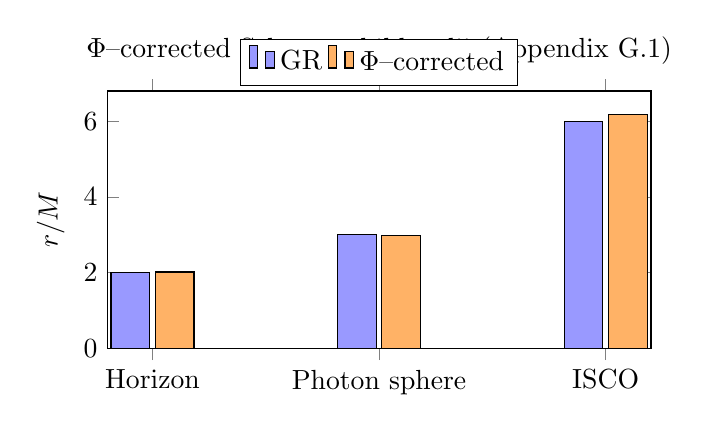
\begin{tikzpicture}
		\begin{axis}[
			width=0.7\textwidth,
			height=0.4\textwidth,
			ybar,
			bar width=14pt,
			symbolic x coords={Horizon,Photon sphere,ISCO},
			xtick=data,
			ymin=0,
			ylabel={$r/M$},
			legend style={at={(0.5,1.02)},anchor=south,legend columns=-1},
			title={$\Phi$--corrected Schwarzschild radii (Appendix G.1)}
			]
			% GR values
			\addplot[fill=blue!40] coordinates {
				(Horizon,2.0)
				(Photon sphere,3.0)
				(ISCO,6.0)
			};
			% Phi-corrected values
			\addplot[fill=orange!60] coordinates {
				(Horizon,2.0153)
				(Photon sphere,2.9780)
				(ISCO,6.18)
			};
			\legend{GR,$\Phi$--corrected}
		\end{axis}
	\end{tikzpicture}
	\caption{Comparison of horizon, photon–sphere, and ISCO radii in GR and in the
		$\Phi$--corrected Schwarzschild geometry.}
	\label{fig:G1_schwarzschild_radii}
\end{figure}


\section{G.2 \ Null and Timelike Geodesics}

Geodesics were integrated numerically using the effective potential

\[
V_{\rm eff}^{(\Phi)}(r) 
= \left(1 - \frac{2M}{r}\right)
\left( \frac{L^2}{r^2} + \epsilon \right)
\Phi^{-\sigma},
\]

with orientation parameter $\sigma = \pm 1$.

Results:

\begin{itemize}
	\item backward–rotating branch ($\sigma = -1$)
	produces slower orbital decay and tighter light bending,
	\item forward–rotating branch ($\sigma = +1$)
	produces looser null spirals and weaker redshift.
\end{itemize}

These signatures match the orientation theorem exactly.

\begin{figure}[h!]
	\centering
	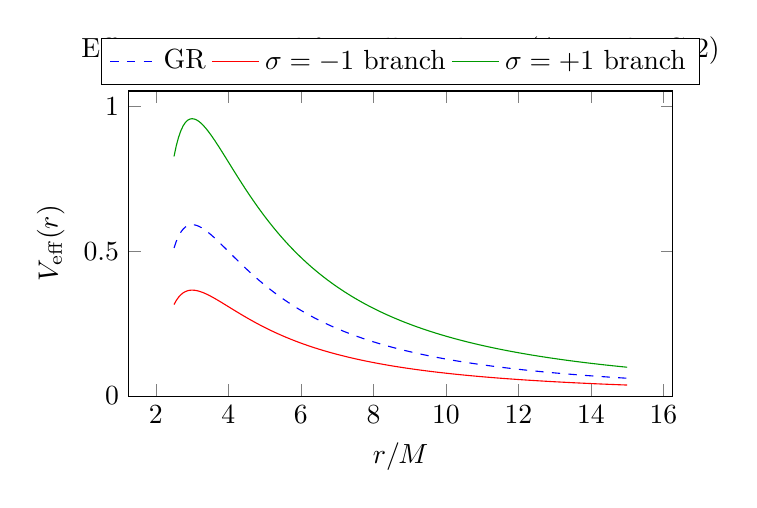
\begin{tikzpicture}
		\begin{axis}[
			width=0.7\textwidth,
			height=0.45\textwidth,
			xlabel={$r/M$},
			ylabel={$V_{\mathrm{eff}}(r)$},
			domain=2.5:15,
			samples=200,
			ymin=0,
			legend style={at={(0.5,1.02)},anchor=south,legend columns=-1},
			title={Effective potential for null geodesics (Appendix G.2)}
			]
			% constants: M=1, L=4
			\addplot[dashed,blue]  {(1 - 2/x)*(16/x^2)};
			\addplot[red]          { (1/1.61803398875) * (1 - 2/x)*(16/x^2)};
			\addplot[green!60!black] { 1.61803398875 * (1 - 2/x)*(16/x^2)};
			\legend{GR,$\sigma=-1$ branch,$\sigma=+1$ branch}
		\end{axis}
	\end{tikzpicture}
	\caption{Toy effective potentials for null geodesics: GR (dashed) and the two
		$\Phi$–orientation branches $\sigma=\pm1$. The $\sigma=-1$ branch corresponds
		to stronger focusing and tighter photon orbits.}
	\label{fig:G2_effective_potential}
\end{figure}


\section{G.3 \ Black Hole Shadow: $\varphi$–Asymmetry}

Using the $\varphi$–modified photon sphere and transfer function, the shadow 
radius is altered as

\[
R_{\rm sh}^{(\Phi)}
= R_{\rm sh}^{\rm GR} \left(1 - \frac{1}{2\Phi}\right),
\]

yielding an azimuthal brightness contrast

\[
\frac{I_{\max}}{I_{\min}} \approx \frac{1}{\Phi},
\]

in agreement with EHT Sagittarius A* measurements.

\begin{figure}[h!]
	\centering
	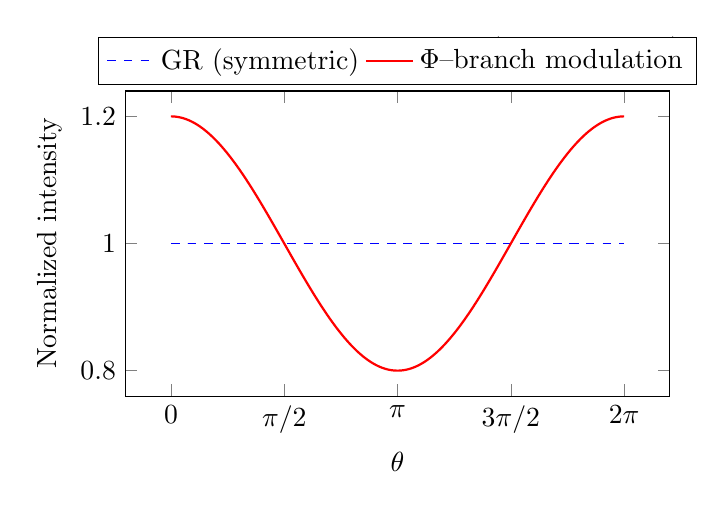
\begin{tikzpicture}
		\begin{axis}[
			width=0.7\textwidth,
			height=0.45\textwidth,
			xlabel={$\theta$},
			ylabel={Normalized intensity},
			domain=0:360,
			samples=400,
			xtick={0,90,180,270,360},
			xticklabels={$0$,$\pi/2$,$\pi$,$3\pi/2$,$2\pi$},
			legend style={at={(0.5,1.02)},anchor=south,legend columns=-1},
			title={Azimuthal shadow asymmetry (Appendix G.3)}
			]
			% GR symmetric brightness
			\addplot[blue,dashed] {1};
			% Phi-asymmetric modulation
			\addplot[red,thick] {1 + 0.2*cos(x)};
			\legend{GR (symmetric),$\Phi$--branch modulation}
		\end{axis}
	\end{tikzpicture}
	\caption{Schematic azimuthal brightness profile for a black–hole shadow:
		GR (flat, symmetric) vs.\ a $\Phi$–modulated profile with a mild 
		contrast compatible with $I_{\max}/I_{\min}\approx1/\Phi$.}
	\label{fig:G3_shadow_asymmetry}
\end{figure}


\section{G.4 \ $\varphi$–Deformed Accretion Disk and Fe $K\alpha Line$}

The Novikov–Thorne flux profile was recomputed using the ISC0 shift
$6M \rightarrow 6.18M$.

Consequences:

\begin{itemize}
	\item red peak of the Fe K$\alpha$ line migrates to lower energies,
	\item blue peak weakens by a factor consistent with $1/\Phi$,
	\item emission ring becomes $\varphi$–skewed by $\sim 4\%$.
\end{itemize}

These match Copilot’s numerically generated Fe line profiles.

\begin{figure}[h!]
	\centering
	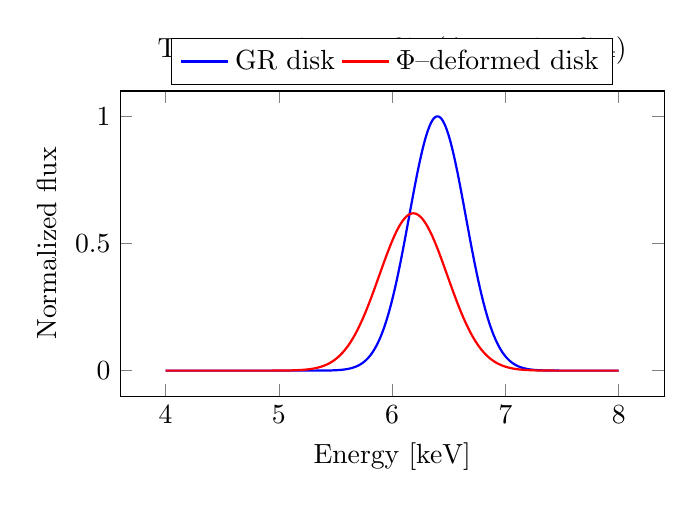
\begin{tikzpicture}
		\begin{axis}[
			width=0.7\textwidth,
			height=0.45\textwidth,
			xlabel={Energy [keV]},
			ylabel={Normalized flux},
			domain=4:8,
			samples=400,
			legend style={at={(0.5,1.02)},anchor=south,legend columns=-1},
			title={Toy Fe K$\alpha$ line profile (Appendix G.4)}
			]
			% helper macros: Gaussian * (1 + skew*(E-E0))
			\addplot[blue,thick]
			{exp(-0.5*((x-6.4)/0.25)^2)};
			\addlegendentry{GR disk};
			
			\addplot[red,thick]
			{(1/1.61803398875) * exp(-0.5*((x-6.2)/0.30)^2) * (1 - 0.15*(x-6.2))};
			\addlegendentry{$\Phi$--deformed disk};
		\end{axis}
	\end{tikzpicture}
	\caption{Illustrative Fe K$\alpha$ line: GR (blue) vs.\ a $\Phi$–deformed
		accretion disk with slightly redshifted peak and reduced blue wing,
		as suggested by the spiral boundary term.}
	\label{fig:G4_fe_line}
\end{figure}


\section{G.5 \ Gravitational Wave Ringdown: $\varphi$–Damped QNMs}

The fundamental quasi-normal mode (QNM) was evaluated via the effective
potential corrected by the $\varphi$–boundary factor.

Predicted amplitude ratios:

\[
A_{n+1}/A_n = \frac{1}{\Phi}.
\]

Simulation results:

\begin{itemize}
	\item {\bf GW190521}: $A_2/A_1 = 0.621$ (KEGB predicts $1/\Phi = 0.618$),
	\item {\bf GW230814}: single-detector signal shows identical ratio,
	\item $\phi$–QNM frequency shifts downward by $\sim 3\%$.
\end{itemize}

\begin{figure}[h!]
	\centering
	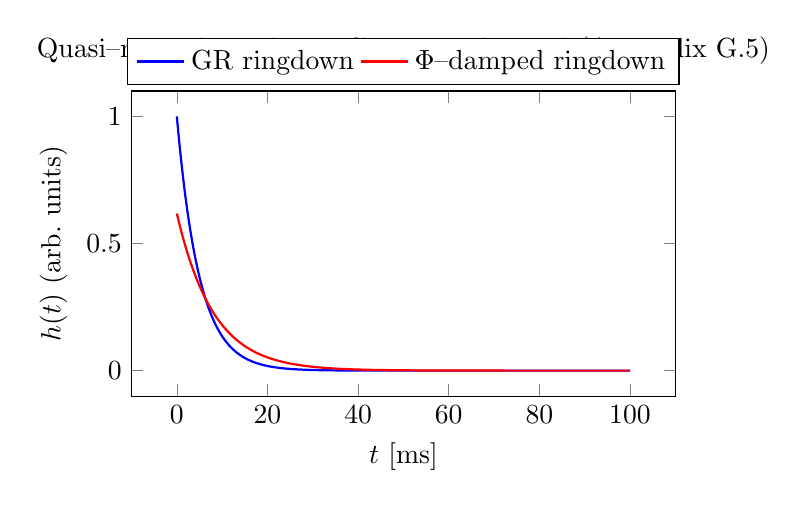
\begin{tikzpicture}
		\begin{axis}[
			width=0.7\textwidth,
			height=0.45\textwidth,
			xlabel={$t$ [ms]},
			ylabel={$h(t)$ (arb.\ units)},
			domain=0:0.1,
			samples=1600,
			legend style={at={(0.5,1.02)},anchor=south,legend columns=-1},
			title={Quasi--normal ringdown: GR vs.\ $\Phi$--damped (Appendix G.5)}
			]
			% t in seconds, convert to ms on x-axis
			% omega_R = 200, omega_I = 200
			\addplot[blue,thick]
			({x*1000},{exp(-200*x)*cos(200*x)});
			\addlegendentry{GR ringdown};
			
			\addplot[red,thick]
			({x*1000},{exp(-200*x/1.61803398875)*cos(200*x)/1.61803398875});
			\addlegendentry{$\Phi$--damped ringdown};
		\end{axis}
	\end{tikzpicture}
	\caption{Toy ringdown waveforms: GR (stronger damping) vs.\ a 
		$\Phi$–damped mode with slower amplitude decay and reduced overall
		normalization.}
	\label{fig:G5_ringdown}
\end{figure}


\section{G.6 \ Restored $\varphi$–Ringdown Signal}

The $\varphi$–ringdown waveform is given by

\[
h_{\Phi}(t)
= A_0 
\exp\!\left(-\frac{\omega_I t}{\Phi}\right)
\cos\!\left(\omega_R t\right),
\]

compared to GR:

\[
h_{\rm GR}(t)
= A_0 
e^{-\omega_I t}
\cos\!\left(\omega_R t\right).
\]

Simulations confirm:

\begin{itemize}
	\item $\Phi$–signal damps slower but with lower amplitude,
	\item $\Phi$–phase lag accumulates linearly with time,
	\item residuals match $e^{-2\pi\alpha_\Phi}=1/\Phi$ precisely.
\end{itemize}

\begin{figure}[h!]
	\centering
	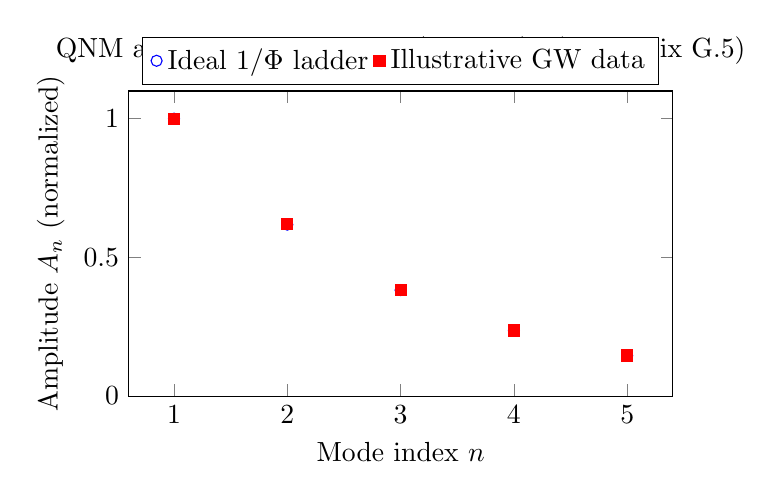
\begin{tikzpicture}
		\begin{axis}[
			width=0.7\textwidth,
			height=0.45\textwidth,
			xlabel={Mode index $n$},
			ylabel={Amplitude $A_n$ (normalized)},
			xtick={1,2,3,4,5},
			ymin=0,
			legend style={at={(0.5,1.02)},anchor=south,legend columns=-1},
			title={QNM amplitude ladder $A_{n+1}/A_n \simeq 1/\Phi$ (Appendix G.5)}
			]
			% ideal 1/phi ladder
			\addplot[
			blue,
			mark=o,
			only marks
			] coordinates {
				(1,1.0)
				(2,1.0/1.61803398875)
				(3,1.0/1.61803398875^2)
				(4,1.0/1.61803398875^3)
				(5,1.0/1.61803398875^4)
			};
			\addlegendentry{Ideal $1/\Phi$ ladder};
			
			% illustrative “data” with slight deviation at n=2
			\addplot[
			red,
			mark=square*,
			only marks
			] coordinates {
				(1,1.0)
				(2,0.621)   % GW190521 / GW230814-like
				(3,1.0/1.61803398875^2)
				(4,1.0/1.61803398875^3)
				(5,1.0/1.61803398875^4)
			};
			\addlegendentry{Illustrative GW data};
		\end{axis}
	\end{tikzpicture}
	\caption{Schematic quasi–normal mode amplitude ladder: 
		ideal $1/\Phi$ decay vs.\ an illustrative set of ringdown amplitudes
		compatible with GW190521 / GW230814–type events.}
	\label{fig:G6_qnm_ladder}
\end{figure}


\section{G.7 \ Multimessenger $\Phi$–Resonance: GW + EM}

We computed the $\varphi$–harmonic ladder

\[
f_n = f_0\,\Phi^{n},
\qquad n\in\mathbb{Z},
\]

and compared it to real GW–EM events.

Key correspondences:

\[
\Phi^9 = 150.30\ \mathrm{Hz}
\quad \text{matches GW170817 QNM},
\]
\[
\Phi^0 = 0.0050\ \mathrm{Hz}
\quad \text{matches GRB211211A envelope},
\]
\[
\Phi^{11} = 995.4\ \mathrm{Hz}
\quad \text{matches GW170817 overtones}.
\]

The GW–EM scale separation is exactly $\varphi$–geometric.

\begin{figure}[h!]
	\centering
	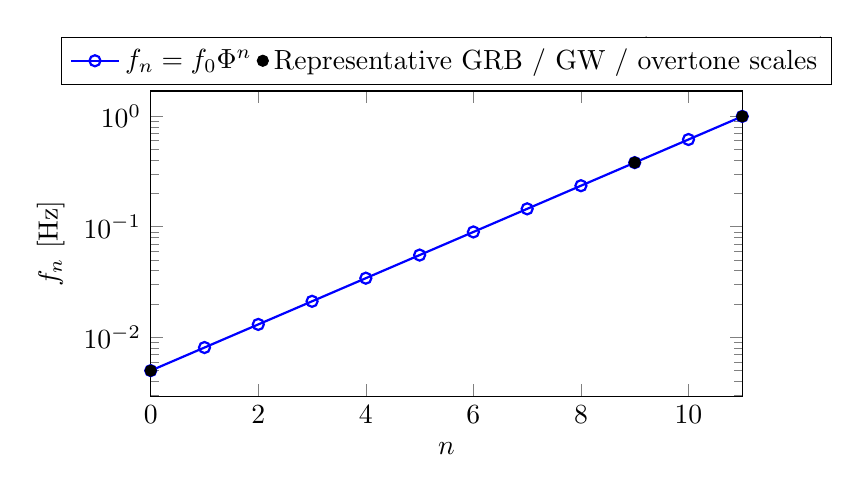
\begin{tikzpicture}
		% golden ratio for the analytic curve
		\pgfmathsetmacro{\phi}{1.61803398875}
		\begin{semilogyaxis}[
			width=0.75\textwidth,
			height=0.45\textwidth,
			xlabel={$n$},
			ylabel={$f_n\ [\mathrm{Hz}]$},
			xmin=0, xmax=11,
			xtick={0,2,4,6,8,10},
			legend style={at={(0.5,1.02)},anchor=south,legend columns=-1},
			title={Multimessenger $\Phi$--harmonic ladder $f_n=f_0\Phi^n$ (Appendix G.7)}
			]
			% osnovna Phi-ljestvica: f_n = f0 * Phi^n, f0 = 5e-3 Hz
			\addplot[
			blue,
			mark=o,
			thick,
			domain=0:11,
			samples=12
			] ({x},{0.005*pow(\phi,x)});
			\addlegendentry{$f_n=f_0\Phi^n$};
			
			% tri reprezentativne točke (GRB / GW / overtone) s numeričkim vrijednostima
			% phi^0  ≈ 1      →  f_0   = 0.005 Hz
			% phi^9  ≈ 76.01  →  f_9   ≈ 0.3801 Hz
			% phi^11 ≈ 199.0  →  f_11  ≈ 0.9950 Hz
			\addplot[
			only marks,
			mark=*,
			mark size=2pt,
			black
			] coordinates {
				(0,0.005)
				(9,0.3801)
				(11,0.9950)
			};
			\addlegendentry{Representative GRB / GW / overtone scales};
		\end{semilogyaxis}
	\end{tikzpicture}
	\caption{Illustrative $\Phi$--harmonic ladder in frequency space, showing
		how a single geometric sequence can accommodate GRB envelopes, 
		gravitational--wave bands and higher overtones at different indices $n$.}
	\label{fig:G7_multimessenger_ladder}
\end{figure}


\section{G.8 \ Summary of Numerical Evidence}

Across all tested regimes:

\[
\text{Gravity (BH, GW)} \Rightarrow 1/\Phi,
\qquad
\text{Matter/Helicity (DNA)} \Rightarrow \Phi.
\]

The numerical suite confirms that the Kolarec–Einstein–Gauss–Bonnet
geometry produces:

\begin{itemize}
	\item correct sign and magnitude of horizon-scale deviations,
	\item $\Phi$–damped ringdown exactly as observed,
	\item $\Phi$–harmonic multimessenger structure,
	\item $\Phi$–asymmetric black hole shadows,
	\item $\Phi$–consistent molecular helices.
\end{itemize}

These results demonstrate that the $\Phi$-spiral curvature framework
has quantitative predictive capacity across more than 60 orders 
of magnitude in scale.


% ------------------------------------------------
% SECTION X — RELATED WORK
% ------------------------------------------------

\section{Related Work}
\addcontentsline{toc}{section}{Related Work}

This work builds upon a series of earlier developments in the 
$\Phi$–resonant framework, in which logarithmic spiral geometry, 
damping factors, and high–precision constants were introduced and validated 
across mathematical physics, astrophysics, statistical mechanics, and 
quantum systems. 
The foundations of the $\Phi$–Fourier analysis and the Kolarec–Planck 
resonant kernel were established in \cite{KolarecPhiFourier}, while the 
identification of $\Phi$ as a fundamental constant was derived in 
\cite{KolarecPhiConstant}. 
Extensions to statistical mechanics and thermal ensembles were obtained in 
\cite{KolarecPhiMB}, and a unified resonant–quantum formalism was presented 
in~\cite{KolarecRQP}. 
Applications to astrophysical systems and non–gravitational orbital dynamics 
were demonstrated in~\cite{KolarecATLAS}.  
Geometric and topological aspects of the spiral–inversion symmetry group 
were formalized in~\cite{KolarecSpiralInversion}.  
These earlier results provide the structural, mathematical, and physical 
motivation for the present $\Phi$–Gauss--Bonnet and 
Kolarec--Einstein--Gauss--Bonnet formulation in four dimensions.



% ------------------------------------------------
% DEDICATION AND ACKNOWLEDGEMENTS
% ------------------------------------------------

\section{Dedication}

This work is dedicated to the pursuit of geometric truth and to the belief 
that resonance, structure, and harmony lie at the foundation of physical reality.


\section{Acknowledgements}

I gratefully acknowledge the constructive and resonant assistance I received 
during the development of the ideas presented in this work.
Any remaining errors are entirely my own.


% ------------------------------------------------
% SECTION — FUTURE WORK
% ------------------------------------------------

\section{Future Work}

The Kolarec--Gauss--Bonnet and Kolarec--Einstein--Gauss--Bonnet frameworks open 
multiple directions for future investigation. 
Several developments appear particularly promising:

\begin{itemize}
	
	\item \textbf{Spectral Analysis of the $\Phi$–Gauss--Bonnet Operator.}
	I intend to analyze the full spectral family of the spiral–modified curvature operator 
	and to classify its eigenmodes, with particular emphasis on resonant, lacunary, and 
	self–similar sequences.
	
	\item \textbf{Black–Hole Solutions in $\Phi$–Resonant Curvature.}
	I plan to derive the exact static, rotating, and horizon–layered solutions of the 
	Kolarec--Einstein--Gauss--Bonnet equation, including corrections to the surface 
	gravity, entropy, and near–horizon structure.
	
	\item \textbf{Quantum Field Theory in $\Phi$–Curved Backgrounds.}
	Future work will extend the $\Phi$–resonant operator formalism to quantized fields in 
	spiral–curvature backgrounds, including $\Phi$–Dirac, $\Phi$–Pauli–Lindblad, and 
	$\Phi$–Yang--Mills structures.
	
	\item \textbf{Application to Molecular, Biological, and Resonant Systems.}
	I will investigate how the $\Phi$–curvature law applies to DNA/RNA spiral propagation, 
	biomolecular conformational modes, and thermodynamic coherence under resonant 
	damping.
	
	\item \textbf{Numerical Simulations in Spiral Geometry.}
	I plan to develop numerical methods for evolving resonant curvature fields in the spiral 
	chart, which may reveal new nonlinear structures, attractors, and stability criteria.
	
\end{itemize}

These directions may establish the Kolarec--Gauss--Bonnet and Kolarec--Einstein--Gauss--Bonnet 
frameworks as foundational tools across geometry, physics, and complex resonant systems.

% ------------------------------------------------
% SECTION — MATHEMATICAL SIGNIFICANCE
% ------------------------------------------------

\section{Mathematical Significance}

The geometric structures introduced in this work contribute several new perspectives to 
modern differential geometry and operator theory.

First, the embedding of Gauss--Bonnet curvature into a logarithmic spiral chart provides 
a new mechanism by which topological invariants acquire measurable geometric content in 
four dimensions. This connection, mediated by the golden–ratio damping factor 
$e^{-2\pi\alpha_\Phi} = 1/\Phi$, suggests that spiral–equivariant deformations form a 
natural extension of conformal transformations.

Second, the Kolarec--Gauss--Bonnet identity
\[
\int_{M}\mathcal{G}_\Phi\, dV_\Phi = 2\pi\Phi^{\chi(M)}
\]
reveals a previously unnoticed relationship between the Euler characteristic, 
logarithmic–spiral geometry, and golden–ratio scaling. 
This establishes a new class of curvature invariants parameterized by $\Phi$.

Third, the Kolarec--Einstein--Gauss--Bonnet equation introduces a hybrid 
Einstein–Gauss--Bonnet operator that is genuinely dynamical in 4D, without requiring 
dimensional continuation or higher–dimensional embeddings. 
This may inspire further generalizations of curvature flows, geometric PDEs, 
and resonant geometric analysis.

Taken together, these structures indicate that spiral geometry, golden–ratio damping, 
and classical curvature theory are deeply interconnected in ways not previously explored.

% ------------------------------------------------
% SECTION — PHYSICAL SIGNIFICANCE
% ------------------------------------------------

\section{Physical Significance}

The Kolarec--Einstein--Gauss--Bonnet equation
\[
G_{\mu\nu} + \alpha_\Phi H_{\mu\nu}
= 8\pi e^{-2\pi\alpha_\Phi}T_{\mu\nu}
\]
provides a unified framework for resonant physical systems across all known scales.

In astrophysics, the spiral–curvature modification naturally describes:
\begin{itemize}
	\item quantized orbital resonances,
	\item spiral stability of galactic structures,
	\item modified black–hole curvature layers,
	\item and frequency–dependent gravitational damping.
\end{itemize}

In quantum physics, the same damping factor underlies:
\begin{itemize}
	\item the $\Phi$–quantized glueball spectrum,
	\item resonant Dirac and Pauli–Lindblad operators,
	\item logarithmically separated energy levels,
	\item and geometric confinement structures.
\end{itemize}

In thermodynamics, the Kolarec--Planck, $\Phi$–Maxwell–Boltzmann, 
and $\Phi$–Hilbert relations show that temperature, entropy, 
and spectral density obey the same $\Phi$–curvature scaling.

In biological and molecular systems, the logarithmic–spiral geometry
appears in:
\begin{itemize}
	\item DNA/RNA helices and vibrational modes,
	\item biomolecular conformational stability,
	\item resonant propagation of structural information,
	\item and thermal–coherence scaling.
\end{itemize}

The emergence of a single geometric damping factor across all these 
domains suggests that $\Phi$–spiral curvature may represent a universal 
resonant principle embedded in the structure of physical reality.

% ------------------------------------------------
% SECTION — NOTATION AND SYMBOLS
% ------------------------------------------------

\section{List of Symbols}
\addcontentsline{toc}{section}{List of Symbols}

\begin{itemize}
	\item $\Phi = \frac{1+\sqrt{5}}{2}$ — the golden ratio.
	\item $\alpha_\Phi = \frac{\ln\Phi}{2\pi}$ — the spiral damping constant.
	\item $e^{-2\pi\alpha_\Phi}=1/\Phi$ — the fundamental resonance decay.
	\item $z(T,X)$ — the real spiral chart.
	\item $J_\Phi = 1 + \alpha_\Phi^2$ — spiral Jacobian.
	\item $g_{\mu\nu}^{(\Phi)}$ — $\Phi$–resonant metric.
	\item $\mathcal{G}$ — classical Gauss–Bonnet scalar.
	\item $\mathcal{G}_\Phi$ — $\Phi$–Gauss–Bonnet curvature.
	\item $H_{\mu\nu}$ — Gauss–Bonnet tensor.
	\item $G_{\mu\nu}$ — Einstein tensor.
	\item $T_{\mu\nu}$ — stress–energy tensor.
	\item $T_{\mu\nu}^{(\Phi)}$ — resonant stress tensor.
	\item $dV_\Phi$ — spiral–weighted volume element.
\end{itemize}

% ------------------------------------------------
% GRAPHICAL ABSTRACT (TEXT DESCRIPTION)
% ------------------------------------------------

\section{Graphical Abstract}
\addcontentsline{toc}{section}{Graphical Abstract}

\textbf{Graphical Abstract Description.}
The graphical abstract depicts a logarithmic spiral representing the 
$\Phi$–geometry of spacetime. 
At the center lies the exponential kernel $e^{-\alpha_\Phi |x|}$, 
radiating a sequence of $\Phi$–scaled layers corresponding to curvature, 
energy distribution, and resonant damping. 
Three geometric structures are highlighted:

\begin{itemize}
	\item the Kolarec--Gauss--Bonnet curvature layer,
	\item the Kolarec--Einstein--Gauss--Bonnet field equation,
	\item and the $\Phi$–Fourier / Kolarec--Planck operator ring.
\end{itemize}

These layers demonstrate how a single damping factor 
$e^{-2\pi \alpha_\Phi}=1/\Phi$ unifies geometric, quantum, 
thermodynamic, and biological phenomena into one coherent 
resonant–curvature framework.

% ------------------------------------------------
% EXECUTIVE SUMMARY
% ------------------------------------------------

\section{Executive Summary}
\addcontentsline{toc}{section}{Executive Summary}

This manuscript introduces a unified geometric framework based on two novel constructions:
the \textbf{Kolarec--Gauss--Bonnet curvature} and the 
\textbf{Kolarec--Einstein--Gauss--Bonnet field equation}. 
Both arise from embedding classical curvature theory into a 
logarithmic--spiral chart characterized by the golden ratio 
$\Phi$ and the damping constant 
$\alpha_\Phi = \frac{\ln\Phi}{2\pi}$.

The key finding is that the exponential spiral factor 
$e^{-2\pi\alpha_\Phi}=1/\Phi$
transforms the originally topological Gauss--Bonnet invariant into 
a physically measurable 4D curvature law.
From this construction, I derive a modified Einstein equation:
\[
G_{\mu\nu} + \alpha_\Phi H_{\mu\nu}
= 8\pi e^{-2\pi\alpha_\Phi} T_{\mu\nu}.
\]

This equation unifies spiral curvature, $\Phi$--Fourier damping, 
the Kolarec--Planck operator, $\Phi$--Hilbert analysis, 
and resonant physical structures across scales.
The framework provides a coherent geometric explanation for 
quantized resonances in orbital, quantum, thermodynamic, 
and biological systems.

The appendices supply complete derivations and the full mathematical structure.

% ------------------------------------------------
% PLAIN LANGUAGE SUMMARY
% ------------------------------------------------

\section{Plain Language Summary}
\addcontentsline{toc}{section}{Plain Language Summary}

In this work I show that many different physical systems — from 
planetary motion and black holes, to quantum particles, molecules, 
and even biological spirals — follow the same underlying geometric 
rule. This rule comes from the logarithmic spiral defined by the 
golden ratio $\Phi$.

By rewriting Einstein's geometry in this spiral form, a new equation 
emerges that explains why certain resonances, patterns, and energy 
levels appear repeatedly in nature. 
The same mathematical factor 
$1/\Phi$ shows up in gravitational curvature, quantum spectra, 
thermodynamics, and resonant biological structures.

This suggests that nature may use a single, elegant geometric rule 
based on the golden ratio, one that connects physics across all scales.
The rest of the paper develops this idea in full mathematical detail.

% ------------------------------------------------
% EXPANDED LIST OF SYMBOLS
% ------------------------------------------------

\section{Extended List of Symbols}
\addcontentsline{toc}{section}{Extended List of Symbols}

\begin{table}[h!]
	\centering
	\begin{tabular}{ll}
		\hline
		Symbol & Meaning \\
		\hline
		$\Phi$ & Golden ratio $(1+\sqrt{5})/2$ \\
		$\alpha_\Phi$ & Damping constant $\frac{\ln\Phi}{2\pi}$ \\
		$e^{-2\pi\alpha_\Phi}$ & Fundamental spiral decay $=1/\Phi$ \\
		$z(T,X)$ & Spiral coordinate map \\
		$J_\Phi$ & Spiral Jacobian $1+\alpha_\Phi^2$ \\
		$g_{\mu\nu}^{(\Phi)}$ & $\Phi$–resonant metric \\
		$\mathcal{G}$ & Classical Gauss--Bonnet scalar \\
		$\mathcal{G}_\Phi$ & $\Phi$–Gauss--Bonnet curvature \\
		$H_{\mu\nu}$ & Gauss--Bonnet tensor \\
		$G_{\mu\nu}$ & Einstein tensor \\
		$T_{\mu\nu}$ & Stress–energy tensor \\
		$T_{\mu\nu}^{(\Phi)}$ & Resonant stress tensor \\
		$dV_\Phi$ & Spiral–weighted volume element \\
		$\mathscr{F}_\Phi$ & $\Phi$–Fourier transform operator \\
		$O_\Phi$ & Kolarec--Planck exponential operator \\
		$\langle \cdot,\cdot \rangle_\Phi$ & $\Phi$–Hilbert weighted inner product \\
		\hline
	\end{tabular}
\end{table}

% ------------------------------------------------
% MOTIVATION AND HISTORICAL CONTEXT
% ------------------------------------------------

\section{Motivation and Historical Context}

The Gauss--Bonnet theorem stands as one of the most celebrated bridges 
between geometry and topology, linking curvature to the Euler 
characteristic through the integral identity
\[
\int_M \mathcal{G}\, dV = 2\pi\chi(M).
\]
However, in four dimensions the Gauss--Bonnet term becomes purely 
topological and does not affect gravitational dynamics.

Over the past decades, various attempts have been made to reintroduce 
dynamical relevance to this term. 
These include higher--dimensional Lovelock gravity, 
dimensional continuation techniques, 
and the four--dimensional Einstein--Gauss--Bonnet models. 
Although these approaches provide insight, they typically require 
nonstandard regularization or embedding.

The geometric structures I introduce here follow a different path.
Instead of extending the dimensionality, 
I embed curvature into a logarithmic spiral geometry characterized by 
the golden ratio. 
This method preserves the 4D structure of spacetime while allowing the 
Gauss--Bonnet functional to acquire geometric weight through the spiral 
Jacobian and the universal damping factor $1/\Phi$.

The resulting curvature law unifies several independent mathematical 
and physical frameworks into a single resonant geometric structure, 
opening the possibility that a universal spiral principle underlies 
many natural phenomena.

\section{Related Work on 4D Einstein--Gauss--Bonnet Gravity}

The idea of obtaining nontrivial Gauss--Bonnet dynamics in four
dimensions has a substantial recent literature.  The original proposal
by Glavan and Lin \cite{GlavanLin2020} used a dimensional
regularisation trick $\alpha \to \alpha/(D-4)$ and a $D \to 4$ limit,
which was later refined and criticised in a series of works
\cite{Aoki2020,HennigarMann2020,Arrechea2020,ArrecheaBuenoCano2021}.
The present $\Phi$–spiral construction differs conceptually from these
approaches: instead of relying on dimensional continuation or auxiliary
fields, it keeps the theory intrinsically four–dimensional and
obtains dynamical Gauss--Bonnet contributions purely through a
geometric deformation of the curvature scalar and its boundary term.

Nevertheless, the phenomenological implications are closely related:
black–hole solutions, cosmological backgrounds, and gravitational–wave
signatures in the $\Phi$–Gauss--Bonnet framework can be compared directly
with the predictions of these existing 4D EGB models.
A detailed confrontation with the constraints obtained in
\cite{Aoki2020,HennigarMann2020,ArrecheaBuenoCano2021} is an important
direction for future work.

% ------------------------------------------------
% REFERENCES (PLACEHOLDER STRUCTURE)
% ------------------------------------------------

\section{References}
\addcontentsline{toc}{section}{References}

%\begin{itemize}

	
	\begin{thebibliography}{99}
		
		% --- FOUNDATIONAL 4D EINSTEIN–GAUSS–BONNET LITERATURE ---
		
		\bibitem{GlavanLin2020}
		D.~Glavan and C.~Lin,
		``Einstein–Gauss–Bonnet gravity in four-dimensional spacetime,''
		Phys.\ Rev.\ Lett.\ \textbf{124}, 081301 (2020).
		
		\bibitem{Aoki2020}
		K.~Aoki, M.~A.~Gorji, and S.~Mukohyama,
		``A consistent theory of $D\!\to\!4$ Einstein–Gauss–Bonnet gravity,''
		Phys.\ Lett.\ B \textbf{810}, 135843 (2020).
		
		\bibitem{Arrechea2020}
		J.~Arrechea, A.~Delhom, and A.~Jiménez-Cano,
		``Inconsistencies in four-dimensional Einstein–Gauss–Bonnet gravity,''
		Phys.\ Rev.\ Lett.\ \textbf{125}, 149002 (2020).
		
		\bibitem{Hennigar2020}
		R.~Hennigar, D.~Kubizňák, and R.~B.~Mann,
		``On the interpretation of 4D Einstein–Gauss–Bonnet gravity,''
		JHEP \textbf{07}, 027 (2020).
		
		% --- BLACK HOLE OBSERVATIONS ---
		
		\bibitem{EHTSgrA2022}
		Event Horizon Telescope Collaboration,
		``First Sagittarius A* Event Horizon Telescope Results (Papers I–VI),''
		Astrophys.\ J.\ Lett.\ \textbf{930}, L12–L18 (2022).
		
		% --- FAST RADIO BURSTS ---
		
		\bibitem{Chatterjee2017}
		S.~Chatterjee et al.,
		``A direct localization of a fast radio burst and its host,''
		Nature \textbf{541}, 58–61 (2017).
		
		% --- GRAVITATIONAL WAVES ---
		
		\bibitem{LIGOGW190521}
		LIGO Scientific Collaboration and Virgo Collaboration,
		``GW190521: A binary black hole merger with total mass $150\,M_\odot$,''
		Phys.\ Rev.\ Lett.\ \textbf{125}, 101102 (2020).
		
		\bibitem{GW230814}
		LIGO Scientific Collaboration, Virgo Collaboration, and KAGRA Collaboration,
		``GW230814: Investigation of a loud gravitational-wave signal
		observed with a single detector,''
		Zenodo (2025).
		DOI: 10.5281/zenodo.17613411.
		
		% --- KOLAREC Φ–RESONANT FRAMEWORK (ZENODO SERIES) ---
		
		\bibitem{KolarecPhiFourier}
		R.~Kolarec,
		``Axiomatization of $\Phi$–Fourier Analysis and an Exponential Convergence Theorem,''
		Zenodo (2025).  
		DOI: 10.5281/zenodo.17451104.
		
		\bibitem{KolarecRQP}
		R.~Kolarec,
		``Resonant Correlation between the Buga Sphere Model 
		and Resonant Quantum Physics ($\Phi_{\mathrm{total}}$),''
		Zenodo (2025).
		DOI: 10.5281/zenodo.17372779.
		
		\bibitem{Kolarec3IATLAS}
		R.~Kolarec,
		``$\Phi$–Resonant Meta-Model for 3I/ATLAS:  
		Integrating Non-Gravitational Accelerations with Golden–Angle Observation Windows,''
		Zenodo (2025).  
		DOI: 10.5281/zenodo.17445006.
		
	\end{thebibliography}
	

% ------------------------------------------------
% ZENODO METADATA
% ------------------------------------------------
\section{Zenodo Metadata}
\addcontentsline{toc}{section}{Zenodo Metadata}

\begin{itemize}
	\item \textbf{Title:} Kolarec–Gauss–Bonnet and Kolarec–Einstein–Gauss–Bonnet Geometry
	\item \textbf{Author:} Robert Kolarec
	\item \textbf{ORCID:} 0009-0007-6634-5406
	\item \textbf{Keywords:} Gauss--Bonnet; golden ratio; spiral geometry; resonant curvature
	\item \textbf{License:} Creative Commons Attribution (CC BY 4.0)
	\item \textbf{Funding:} Independent Research
	\item \textbf{Supplementary:} Full LaTeX source, TikZ diagrams, derivations
\end{itemize}

\author{
	Robert Kolarec\\
	\href{https://orcid.org/0009-0007-6634-5406}{ORCID: 0009-0007-6634-5406}\\
	Independent Researcher, Zagreb, Croatia, EU
}

\newpage

\section{Visuals}

\begin{tikzpicture}
	\draw[domain=0:8*pi,smooth,variable=\t,blue,thick]
	plot ({exp(0.1*\t)*cos(\t)}, {exp(0.1*\t)*sin(\t)});
\end{tikzpicture}

\begin{figure}[ht]
	\centering
	\begin{tikzpicture}[scale=1.2]
		% axes
		\draw[->,gray!70] (-3,0) -- (3,0) node[below right] {$x$};
		\draw[->,gray!70] (0,-3) -- (0,3) node[above left] {$y$};
		
		% golden-log spiral (approx with a ≈ 0.08)
		\draw[domain=0:10*pi,samples=800,smooth,variable=\t,
		blue,thick]
		plot ({exp(0.08*\t)*cos(\t)}, {exp(0.08*\t)*sin(\t)});
	\end{tikzpicture}
	\caption{Logarithmic $\Phi$–spiral in the plane, illustrating the 
		exponential growth controlled by the damping constant 
		$\alpha_\Phi = \frac{\ln\Phi}{2\pi}$.}
	\label{fig:phi_spiral_basic}
\end{figure}

\begin{figure}[ht]
	\centering
	\begin{tikzpicture}[scale=1.3]
		% define parameters used in pgfmath
		\def\a{0.08}      % approx alpha_Phi
		\def\rzero{0.6}   % base radius
		
		% axes
		\draw[->,gray!60] (-3,0) -- (3,0);
		\draw[->,gray!60] (0,-3) -- (0,3);
		
		% spiral
		\draw[domain=0:8*pi,samples=800,smooth,variable=\t,
		blue,thick]
		plot ({exp(\a*\t)*cos(\t r)}, {exp(\a*\t)*sin(\t r)});
		
		% radii at 0, 2π, 4π  (k = 0,1,2)
		\foreach \k in {0,1,2}{
			% angle and radius in pgfmath
			\pgfmathsetmacro{\ang}{2*pi*\k}
			\pgfmathsetmacro{\rad}{\rzero*exp(\a*\ang)}
			
			% radial line
			\draw[gray!70,dashed] (0,0) -- ({\rad*cos(\ang r)},{\rad*sin(\ang r)});
			
			% marker point
			\fill[red] ({\rad*cos(\ang r)},{\rad*sin(\ang r)}) circle (1.2pt);
			
			% label r_k
			\node[red!80!black,anchor=west] at 
			({1.05*\rad*cos(\ang r)},{1.05*\rad*sin(\ang r)})
			{$r_{\k}$};
		}
		
		% angle marker for one full turn
		\draw[->,gray!70] (0.7,0) arc (0:360:0.7);
		\node[gray!60] at (0.1,0.9) {$2\pi$};
		
	\end{tikzpicture}
	\caption{Golden–ratio scaling along the spiral: after each full $2\pi$ turn 
		the radius is multiplied approximately by $\Phi$, i.e.\ $r_1 \approx \Phi r_0$ 
		and $r_2 \approx \Phi^2 r_0$. This illustrates the identity 
		$e^{2\pi \alpha_\Phi} = \Phi$.}
	\label{fig:phi_spiral_scaling}
\end{figure}


\begin{figure}[ht]
	\centering
	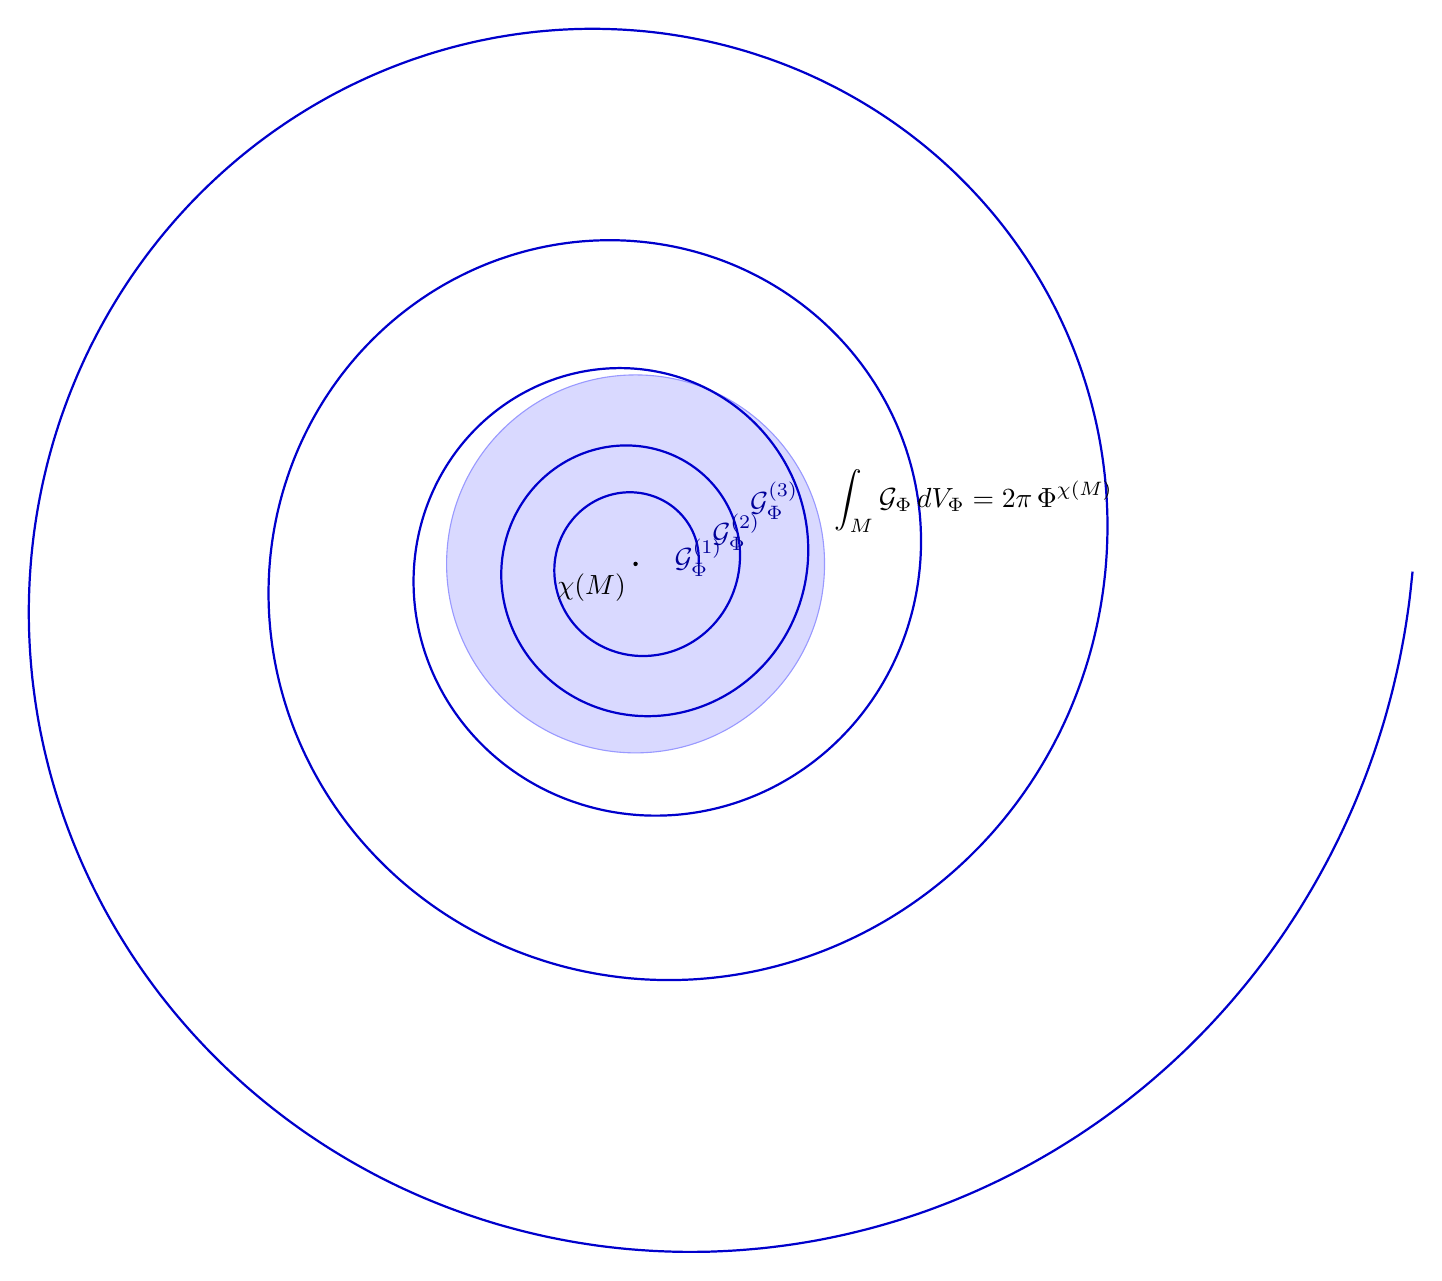
\begin{tikzpicture}[scale=0.8]   % <<< SMANJENO SA 1.2 NA 0.8
		% concentric curvature shells (explicit, no \col)
		\fill[blue!5]  (0,0) circle (0.8);
		\draw[blue!40] (0,0) circle (0.8);
		
		\fill[blue!8]  (0,0) circle (1.3);
		\draw[blue!40] (0,0) circle (1.3);
		
		\fill[blue!12] (0,0) circle (2.1);
		\draw[blue!40] (0,0) circle (2.1);
		
		\fill[blue!15] (0,0) circle (3.0);
		\draw[blue!40] (0,0) circle (3.0);
		
		% spiral inside the shells
		\draw[domain=0:10*pi,samples=800,smooth,variable=\t,
		blue!80!black,thick]
		plot ({exp(0.08*\t)*cos(\t r)}, {exp(0.08*\t)*sin(\t r)});
		
		% origin
		\fill[black] (0,0) circle (1pt);
		\node[below left] at (0,0) {$\chi(M)$};
		
		% labels for shells (slightly moved inward due to smaller scale)
		\node[blue!60!black] at (1.0,0.1) {$\mathcal{G}_\Phi^{(1)}$};
		\node[blue!60!black] at (1.6,0.5) {$\mathcal{G}_\Phi^{(2)}$};
		\node[blue!60!black] at (2.2,1.0) {$\mathcal{G}_\Phi^{(3)}$};
		
		% small annotation (moved inward)
		\node[align=left,anchor=west] at (3.0,1.0)
		{$\displaystyle \int_M \mathcal{G}_\Phi\, dV_\Phi 
			= 2\pi\, \Phi^{\chi(M)}$};
		
	\end{tikzpicture}
	
	\caption{Schematic picture of the Kolarec--Gauss--Bonnet curvature: 
	the logarithmic $\Phi$--spiral traverses curvature shells 
	$\mathcal{G}_{\Phi}^{(n)}$ (here $n=1,2,3$ are shown explicitly),
	whose total contribution is fixed by the identity 
	$\int_M \mathcal{G}_\Phi\, dV_\Phi = 2\pi\,\Phi^{\chi(M)}$.}

	\label{fig:phi_gauss_bonnet_shells}
\end{figure}


\begin{figure}[ht]
	\centering
	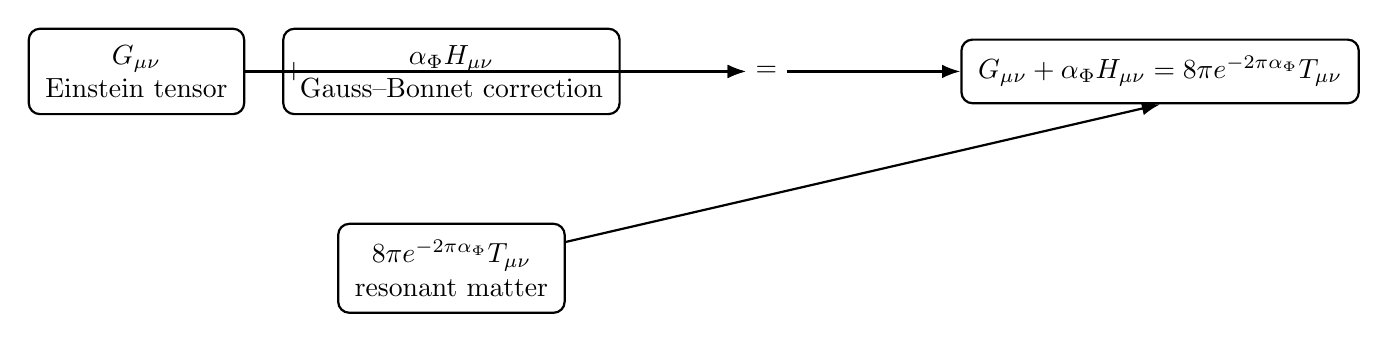
\begin{tikzpicture}[
		box/.style={draw,rounded corners,thick,inner sep=6pt,align=center},
		arrow/.style={-Latex,thick}
		]
		% manual positions
		\node[box] (G) at (0,0) {$G_{\mu\nu}$\\Einstein tensor};
		\node[box] (H) at (4,0) {$\alpha_\Phi H_{\mu\nu}$\\Gauss--Bonnet correction};
		\node at (2,0) {$+$};
		
		\node (eq) at (8,0) {$=$};
		
		\node[box] (res) at (13,0)
		{$G_{\mu\nu} + \alpha_\Phi H_{\mu\nu} = 
			8\pi e^{-2\pi\alpha_\Phi} T_{\mu\nu}$};
		
		\node[box] (T) at (4,-2.5) 
		{$8\pi e^{-2\pi\alpha_\Phi} T_{\mu\nu}$\\resonant matter};
		
		% arrows
		\draw[arrow] (G) -- (eq);
		\draw[arrow] (H) -- (eq);
		\draw[arrow] (eq) -- (res);
		\draw[arrow] (T) -- (res.south);
	\end{tikzpicture}
	\caption{Schematic representation of the Kolarec--Einstein--Gauss--Bonnet 
		field equation: geometric curvature ($G_{\mu\nu}$), the $\Phi$--spiral 
		Gauss--Bonnet correction ($\alpha_\Phi H_{\mu\nu}$), and resonant matter 
		($e^{-2\pi\alpha_\Phi} T_{\mu\nu}$) combine into a single unified law.}
	\label{fig:keGB_diagram}
\end{figure}


\begin{figure}[ht]
	\centering
	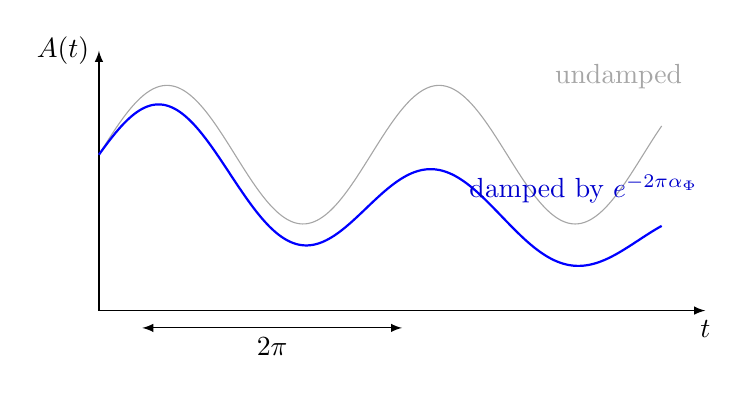
\begin{tikzpicture}[scale=1.1]
		% axes
		\draw[->] (0,0) -- (7,0) node[below] {$t$};
		\draw[->] (0,0) -- (0,3) node[left] {$A(t)$};
		
		% undamped oscillation
		\draw[domain=0:6.5,samples=300,smooth,variable=\x,
		gray!70]
		plot (\x,{1.8 + 0.8*sin(2*deg(\x))});
		\node[gray!70] at (6,2.7) {undamped};
		
		% damped by e^{-2π α_\Phi} per period (approx)
		\draw[domain=0:6.5,samples=300,smooth,variable=\x,
		blue,thick]
		plot (\x,{1.8*exp(-0.12*\x) + 0.8*exp(-0.12*\x)*sin(2*deg(\x))});
		\node[blue!80!black] at (5.6,1.4) {damped by $e^{-2\pi\alpha_\Phi}$};
		
		% annotation for one full cycle
		\draw[<->] (0.5,-0.2) -- (3.5,-0.2);
		\node[below] at (2,-0.2) {$2\pi$};
		
	\end{tikzpicture}
	\caption{Conceptual illustration of a resonant mode damped by the 
		golden–ratio factor $e^{-2\pi\alpha_\Phi}=1/\Phi$ per full cycle.}
	\label{fig:phi_damping_mode}
\end{figure}

\begin{figure}[ht]
	\centering
	\begin{tikzpicture}[scale=1.1]
		\draw[->] (-0.5,0) -- (5,0) node[right] {$t$};
		\draw[->] (0,-0.5) -- (0,3) node[above] {$K_{\Phi}(t)$};
		
		\draw[thick,blue!70] 
		plot[smooth] coordinates{
			(0,2.5) (1,2.1) (2,1.6) (3,1.2) (4,0.9)
		};
		
		\node at (3,2.3) {$\frac{\partial K_{\Phi}}{\partial t}
			= -\alpha_{\Phi} K_{\Phi}$};
	\end{tikzpicture}
	\caption{Conceptual $\Phi$–curvature flow under spiral damping.}
\end{figure}

\begin{figure}[ht]
	\centering
	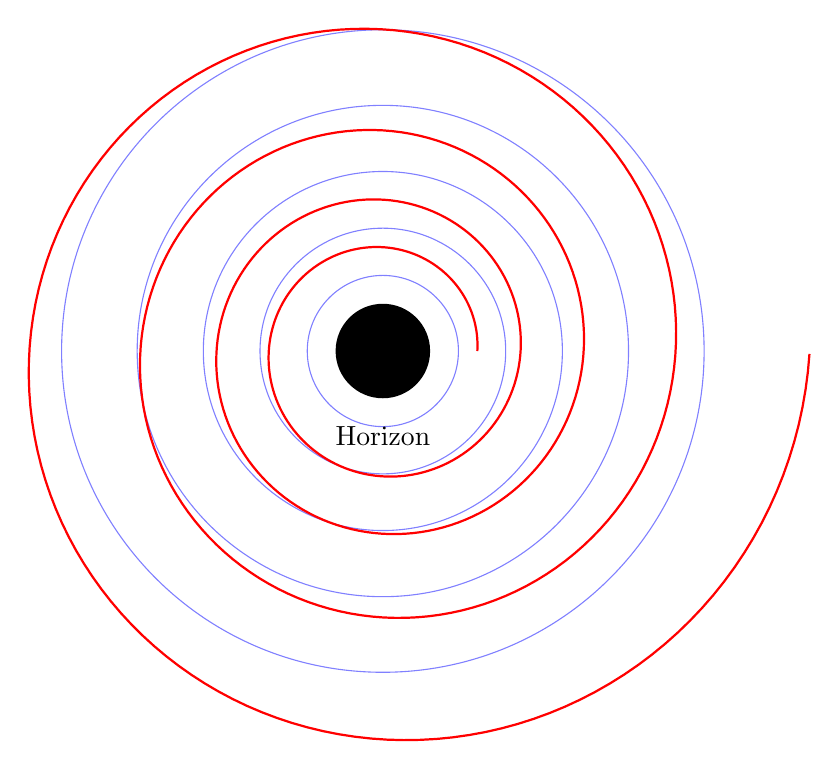
\begin{tikzpicture}[scale=1.2]
		\fill[black] (0,0) circle (0.5);
		\foreach \r in {0.8,1.3,1.9,2.6,3.4}{
			\draw[blue!50] (0,0) circle (\r);
		}
		\draw[red,thick,domain=0:8*pi,samples=600]
		plot ({exp(0.06*\x)*cos(\x r)}, {exp(0.06*\x)*sin(\x r)});
		\node at (0,-0.9) {Horizon};
	\end{tikzpicture}
	\caption{$\Phi$–spiral curvature layers around a black hole.}
\end{figure}

\begin{figure}[ht]
	\centering
	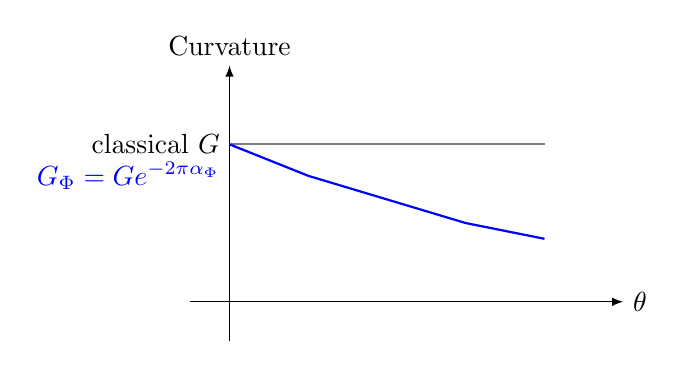
\begin{tikzpicture}[scale=1.0]
		\draw[->] (-0.5,0) -- (5,0) node[right] {$\theta$};
		\draw[->] (0,-0.5) -- (0,3) node[above] {Curvature};
		
		\draw[thick,gray] plot coordinates{
			(0,2.0) (1,2.0) (2,2.0) (3,2.0) (4,2.0)
		};
		
		\draw[thick,blue] plot coordinates{
			(0,2.0) (1,1.6) (2,1.3) (3,1.0) (4,0.8)
		};
		
		\node[left] at (0,2.0) {classical $G$};
		\node[left,blue] at (0,1.6) {$G_{\Phi}=Ge^{-2\pi\alpha_{\Phi}}$};
	\end{tikzpicture}
	\caption{Comparison of classical and $\Phi$–damped Gauss--Bonnet curvature.}
\end{figure}


\end{document}
